\documentclass[
11pt, english, singlespacing,
headsepline,
chapterinoneline,
%consistentlayout, 
]{MastersDoctoralThesis}

% Load packages

%\usepackage{unicode-math}
%\setmainfont[
%  Extension=.otf,
%  UprightFont={*-Regular},
%  BoldFont={*-Bold},
%  ItalicFont={*-Italic},
%  BoldItalicFont={*-BoldItalic}
%]{LibertinusSerif}

\usepackage[utf8]{inputenc} % Required for inputting international characters
\usepackage[T1]{fontenc} % Output font encoding for international characters
\usepackage{mathpazo}
\usepackage{libertine} % Use the Palatino font by default

\usepackage[url=false, backend=biber, style=numeric]{biblatex} % Use the bibtex backend with the authoryear citation style (which resembles APA)
\addbibresource{Bibliography/bibliography.bib} % The filename of the bibliography

\usepackage[autostyle=true]{csquotes} % Required to generate language-dependent quotes in the bibliography


%\usepackage[font=small]{caption}
\usepackage{afterpage}
\usepackage{graphicx}
\usepackage{ragged2e}
\usepackage{verbatim}
\usepackage{latexsym}
\usepackage{setspace}
\usepackage{float}
\usepackage{subcaption}
\usepackage{url}
\usepackage{hyperref}
\hypersetup{
     colorlinks=true,
     linkcolor=black,
     filecolor=black,
     citecolor=black,
     urlcolor=black,
}     
\usepackage{tabularx}
\usepackage{booktabs}
\usepackage{multirow}
\usepackage[normalem]{ulem}
\usepackage{pdfpages}
\usepackage[htt]{hyphenat}
\usepackage[acronym]{glossaries}
\usepackage{enumitem}
\usepackage{amsmath}
\usepackage{changepage}
\usepackage{textcomp, amssymb, amsfonts, romannum, bbm, amsthm, enumerate}
\usepackage{wrapfig}

% Margins
\geometry{
	paper=a4paper, % Change to letterpaper for US letter
	inner=2.5cm, % Inner margin
	outer=3.8cm, % Outer margin
	bindingoffset=.5cm, % Binding offset
	top=1.5cm, % Top margin
	bottom=1.5cm, % Bottom margin
	%showframe, % Uncomment to show how the type block is set on the page
}

% Information
\newcommand{\thesistype}{Mini-Thesis}
\newcommand{\titel}{Development and investigation of general non-linear framework for solving rotation-free solid membranes}
\newcommand{\autor}{Harsh Pandey}
\newcommand{\matnumber}{415518}
\newcommand{\studyprogram}{M.Sc. CAME}

\newcommand{\supervisorinternal}{Michal Rajski M.Sc.}
%\newcommand{\supervisorexternal}{Max Mustermann, B.Sc.}
\newcommand{\submitdate}{10\textsuperscript{th} of October 2022}


\newcommand\blankpage{%
	\null
    \thispagestyle{empty}%
    \addtocounter{page}{-1}%
    \newpage}

\begin{document}

\frontmatter % Use roman page numbering style (i, ii, iii, iv...) for the pre-content pages

\pagestyle{plain} % Default to the plain heading style until the thesis style is called for the body content

% Title page
\begin{titlepage}
	
	\begin{center}
		
		\vspace*{-2cm}
		\begin{minipage}[b]{0.45\textwidth}
		\end{minipage}
		\hfill
		\begin{minipage}[b]{0.45\textwidth}
		\begin{flushright}
					
\includegraphics[height=6em]{Style/rwth_km_logo_en.eps}
		\end{flushright}
		\end{minipage}
		
		%\normalsize{\scshape{
		%		The present work was submitted to the Department of Continuum Mechanics}
		%}\\[1em]
		%\vspace{1cm}
		%\normalsize{\scshape\textbf{Rheinisch-Westfälische Technische Hochschule Aachen}}\\
		%\normalsize{\normalfont\scshape{Faculty of Mechanical Engineering}}
		
		\normalsize{{
				The present work was submitted to the Department of Continuum Mechanics}
		}\\[1em]
		\vspace{1cm}
		\normalsize{\textbf{Rheinisch-Westfälische Technische Hochschule Aachen}}\\
		\normalsize{\normalfont{Faculty of Mechanical Engineering}}
		
		\vspace{2cm}
		
		%\Large{\scshape\textbf{\thesistype}}\\[4ex]
		%\huge{\textbf{\titel}}\\[1.5ex]
		%\huge{\scshape\textbf{\titel}}\\[1.5ex]

		\Large{\textbf{\thesistype}}\\[4ex]
		%\huge{\textbf{\titel}}\\[1.5ex]
		\huge{\textbf{\titel}}\\[1.5ex]
		
		\vfill{}
		
		\normalsize
		\begin{tabular}{p{5cm}p{8cm}}
			Presented by: 			& \quad  \autor\\[1.2ex]
			Study programme:		& \quad  \studyprogram\\[1.2ex]
			Matriculation number: 	& \quad \matnumber\\[1.2ex]
			Reviewer: 				& \quad Univ.-Prof. Dr.-Ing. Mikhail Itskov\\[1.2ex]
			Supervisor:				& \quad \supervisorinternal \\[1.2ex]
			%External supervisor:	& \quad \supervisorexternal \\[1.2ex]
		\end{tabular}
		
		\vspace{3cm}
		
		Aachen, \submitdate
		
		\vspace*{-3.3cm}
		
	\end{center}
	
\end{titlepage}
\newpage


% Declaration page
\include{FrontBackMatter/Authorship}

% Abstract
%\include{FrontBackMatter/Abstract}

% Acknowledgements
%\include{FrontBackMatter/Acknowledgements}

%	Include table content, list of figures and of tables
\include{FrontBackMatter/ListOfContent}

% List of symbols, abbreviations and constants
%\include{FrontBackMatter/Symbols}


% Content
\mainmatter % Begin numeric (1,2,3...) page numbering
\pagestyle{thesis} % Return the page headers back to the "thesis" style

% Chapter 1
\chapter{Introduction to Shells} % Main chapter title

\label{Chapter1} % For referencing the chapter elsewhere, use \ref{Chapter1} 

%----------------------------------------------------------------------------------------

% Define some commands to keep the formatting separated from the content 
\newcommand{\keyword}[1]{\textbf{#1}}
\newcommand{\tabhead}[1]{\textbf{#1}}
\newcommand{\code}[1]{\texttt{#1}}
\newcommand{\file}[1]{\texttt{\bfseries#1}}
\newcommand{\option}[1]{\texttt{\itshape#1}}

%----------------------------------------------------------------------------------------
\section{What are shells and membranes?}
Most structural objects and elements can be reduced to a physical line with a certain cross-section. The description of stresses
 in these objects can be done by describing  “stress resultants” - the normal force, transverse shearing forces, bending
 moments, and the torque - in the cross section. In contrast to these objects, certain structural elements enclose some space making it impossible for them to be reduced to a line. They are better described as a curved surface
 or a plane. These elements can be broadly broken down in two categories - plates and shells \cite{flugge2013}.

A shell is a curved, thin-walled structure with the thickness being significantly smaller than the other dimensions \cite{bischoff2004}.
 The distinguishing feature between a shell and a plate is that the shell has a curvature whereas plates are flat
 structures \cite{chen1997}. It is, however, not necessary for the thickness in a shell to be extremely small. It can also vary across
 the surface. The behaviour of a shell can be geometrically linear or nonlinear. Membranes are special cases of shells whose walls offer
 no resistance to bending moments and transverse shear forces. 

Shells carry load efficiently - this is most optimally done when all the load is carried using membrane forces; 
 exhibit high structural integrity, strength to weight ratio; and have high stiffness \cite{ventsel2001}.
 Shells and membranes are ubiquitous in engineering and nature because of the advantages they present - from aerospace as
 aeroplanes and rocket hulls, civil engineering where they are found in large span roofs, cooling towers, containment
 tanks, to biological systems such as skulls, eyes, cells, and blood vessels.
%----------------------------------------------------------------------------------------
%----------------------------------------------------------------------------------------
\section{Problems with modelling shells/membranes}
In the real world, thin shells are very sensitive to imperfections and can be highly unstable if not designed properly \cite{loibl2019}.
 Modelling this complexity is challenging too. Shells can undergo large deformations, large rotations, and large strains.
 They can behave highly nonlinearly and can have multiple instabilities - in compression, for out-of-plane loading, for 
 pressure loading, and with respect to in-plane loading \cite{sauer2014}.
 This mixture of performance and sensitivity makes the shell the 'primadonna of structures' \cite{bischoff2004}. Given that there are
 no analytical solutions for most cases to predict a shell's behaviour, reliable approximate solutions are necessary.

Shell theories aim to reduce the dimensionality of the equilibrium problem from a 3D body to only the study of the
 midsurface of the shell. This dimensionality reduction is often dependent on the thickness of shells. Generally, shells
 with a thickness h and general radius of curvature R, can be categorised as thin shells if $\text{max}(h/R)<=(1/20)$.
Love laid the foundations of classical linear shell theory by applying the Kirchhoff hypothesis to thin,
 homogenous, isotropic, linear-elastic shells governed by a generalised Hooke's law. Known as the Kirchhoff-Love theory,
 the assumptions can be summarised as \cite{podio1989}:
\begin{itemize}
    \item No deformation in the midsurface - it is the neutral plane during bending.
    \item Points that lie on the normal to the midsurface remain so even after deformation.
\end{itemize}
The transverse normal stresses and the transverse shear strains are neglected. 
Reissner \cite{reissner1941} and Mindlin \cite{mindlin1951} separately expanded upon the Kirchhoff-Love hypothesis with the inclusion of transverse shear
strains and first order shear effects in their derivations, which could calculate the deformation of shells with a
thickness of $\text{max}(h/R) <= (1/10)$. Their theories assumed the following:
\begin{itemize}
    \item The normals of the undeformed midsurface are deformed into the normals to the deformed midsurface.
    \item The stress components normal to the middle surface are small compared to the other stress components and can be neglected in the stress-strain relations
    \item The displacements are so small that the equilibrium conditions for deformed elements are the same as if they were not deformed.
\end{itemize}
There is a lack of a universally accepted classical linear shell theory, all of which share a degree of inaccuracy
 due to their arbitrary treatment of secondary effects \cite{nayfeh2004} and \emph{ad hoc} assumptions \cite{naghdi1963}
 during different stages of the formulation of the governing equations. Love's first
 approximation
 \begin{itemize}
    \item doesn't satisfy the equilibrium equation arising from the symmery of the stress tensor,
    \item isn't invariant under infinitesimal rigid body displacement and,
    \item violates a 2D analogue of the Betti-Rayleigh reciprocity theorem in 3D linear elasticity.
\end{itemize}
Reissner's first approximation runs into the same problems except violating the reciprocity theorem \cite{truesdell1984}. Although improvements to classical linear
 shell theories can be found in later works by Reissner (1959), Novozhilov (1959), Sanders (1959), and Koiter
 (1959), Naghdi \cite{naghdi1963} mentions the existence of inconsistencies present in many of these approximations. 

The formulation presented in this report is based on the work of Sauer \cite{sauer2014}, which is a formulation of
 the theoretical framework laid down by Steigmann \cite{steigmann1999}. Although substantially same as Naghdi's \cite{truesdell1984}
 formulation, Steigmann's assumptions logically conform to finite elasticity theory. Sauer's formulation is also specifically based on
 membranes because while membranes are special cases of shells and a formulation for shells could be extended to membranes, a formulation dedicated explicitly
 towards membranes is more robust and accurate \cite{sauer2014}. Here, liquid membranes can also be accounted for through the
 split of contributions between the in-plane and out-of-plane components, admission of arbitrary elastic material models,
 all quantities are formulated directly in curvilinear coordinates.

The following chapter presents the theory and formulation of the finite element method for the solution of an elliptic
 boundary vaue problem. Chapter 3 details the theory and implementation of the finite element method to nonlinear boundary
 value problems for solid mechanics in an orthonormal basis system. Chapter 4 extends this nonlinear framework to membranes
 through the incorporation of curvilinear coordinates and presents numerical examples to illustrate the capabilities of the
 formulation.
%----------------------------------------------------------------------------------------
\afterpage{\blankpage}

% Chapter 2

\chapter{Finite Element Method} % Main chapter title

\label{Chapter2} % For referencing the chapter elsewhere, use \ref{Chapter1} 

%----------------------------------------------------------------------------------------
%----------------------------------------------------------------------------------------

\newtheorem{definition}{Definition}[section]

\section{Introduction: Poisson Problem} \label{sec:poisson_weak_form}
The Poisson equation is the simplest and the most famous elliptic partial differential equation \cite{arbenz2017}.
Considering a Poisson problem posed in a domain $\mathcal{D}$, a bounded subset of $\mathbb{Rd}$, with prescribed boundary conditions, the problem can be defined in its entirety as:
\begin{equation} \label{def_poisson}
    \begin{cases}
        \nabla ^{2}  u = s  & \text{in $\mathcal{D}$}\\
        u = \overline{u}  & \text{on $\mathcal{S}_{u}$}\\
        q = \frac{\partial u}{\partial x} \cdot \boldsymbol{n} = \overline{q} & \text{on $\mathcal{S}_{q}$},
    \end{cases}
\end{equation}
where \emph{u} defines the unknown potential, $\overline{u}$ is the prescribed value of potential on $\mathcal{S}_{u}$ portion of the boundary and $\overline{q}_{q}$ is the prescribed flux on $\mathcal{S}_{q}$
 with $\mathcal{S} = \mathcal{S}_{u} \cup \mathcal{S}_{q}$ being the boundary of the domain $\mathcal{D}$. The source term is denoted as \emph{s}.
 Equation \eqref{def_poisson} is referred to as a boundary value problem. If $\mathcal{S}_{q} = \emptyset$, the problem is referred to as a Dirichlet problem.
 Similarly, if $\mathcal{S}_{u} = \emptyset$, the problem is called a Neumann problem.
 A third possibility exists for when there's both a prescribed flux and a prescribed value of the potential on disjointed subsets of the boundary such that $\mathcal{S} = \mathcal{S}_{q} \cup \mathcal{S}_{u}$.

A sufficiently smooth function \emph{u} satisfying \eqref{def_poisson} is known as a \emph{classical solution} to the boundary value problem \cite{arbenz2017}.
 This puts a strong condition on \emph{u} to be atleast twice differentiable in the domain $\mathcal{D}$.
However, due to discontinuous source functions or a discontinuous domain, the existence of a classical solution might not be possible.
This is not uncommon and necessitates an alternative description of the boundary value problem
 - called the \emph{weak formulation} as it reduces the constraints imposed upon the solution.
To achieve this two functional spaces must be defined. The space of test functions,
\begin{equation} \label{test_space}
    \mathcal{V} = \{
        w \in H^{1}_{0}(\mathcal{D}) \, | \, \, w = 0 \ \text{on $\mathcal{S}_{u}$}
        \}
\end{equation}
and the space of collection of functions known as trial solutions
\begin{equation} \label{solution_space}
    \mathcal{W} = \{
        u \in H^{1}(\mathcal{D}) \, | \,\, u = \overline{u} \ \text{on $\mathcal{S}_{u}$}.
        \}
\end{equation}
%
Based on the weighted residual method, using these test functions and using the product rule on the right hand side, we get
\begin{align*}
    (s, w) := \int_{\mathcal{D}}  w\, s\,\, dv &= \int_{\mathcal{D}} w \, \nabla^{2} u \,dv\\
    &= \int_{\mathcal{D}}[\nabla(w \, \nabla u) - \nabla w \, \nabla u] \,dv.
\end{align*} 
Applying the divergence theorem,
\begin{equation}
    \int_{\mathcal{D}} \nabla(w \, \nabla u) \,dv = \int_{\mathcal{S}} w (\nabla u \cdot \boldsymbol{n}) \,da
\end{equation}
and substituting the result in the previous equation,
\begin{equation} \label{weak_formulation_1}
    -\int_{\mathcal{D}} \nabla w \cdot \nabla u \, \,dv + 
        \int_{\mathcal{S}} w \,(\nabla u \cdot \boldsymbol{n} \,da)  =  \int_{D} w \, s \, \,dv.
\end{equation}
As $w = 0$ on $\mathcal{S}_{u}$ and according to the problem statement and the definition of Neumann boundary conditions, equation
 \eqref{weak_formulation_1} can be written as
\begin{equation} \label{weak_formulation_2}
    - \int_{\mathcal{D}} \nabla w \cdot \nabla u \, \,dv = \int_{\mathcal{D}} w \, s \,\,dv - \int_{\mathcal{S}_{q}} w \, \overline{q} \,\,da.
\end{equation}

\subsection{Function Spaces and Well-Posedness of the Weak Formulation} 
For the equality in \eqref{weak_formulation_2} to make sense, it is no longer necessary for \emph{u} to be twice differentiable. The classical definition of a derivative
 is stated pointwise - thus requiring the function to be defined at all points. For \eqref{def_poisson}, this implies that \emph{u} be $C^{2}$ continuous. The weak derivative involed in the weak formulation is more general and includes functions that
 that are not necessarily $C^{2}$ contininuous throughout the domain. This requires the definition of a function space where it is possible to define a weak derivative.
 This function space is where the \emph{test functions} and \emph{trial solutions} live. This function space is called a \emph{Sobolev space}. 
 Using the space of square integrable functions,
 \begin{equation} \label{square_integrable_space}
    L^{2}(\Omega) = \left\{f: \Omega \to \mathbb{R} : \int_{\Omega} |f|^{2} < \infty \right\},
 \end{equation} 
 the Sobolev spaces for a given $f \in L^{2}(\Omega)$ can be defined as
\begin{equation}\label{sobolev_space}
    H^{1}(\Omega) = \left\{f \in L^{2}(\Omega): \frac{\partial f}{\partial x_{1}}, \frac{\partial f}{\partial x_{2}} \in L^{2}(\Omega)\right\}.
\end{equation}
and,
\begin{equation} \label{hilbert_space}
    H^{1}_{0}(\Omega) = \left\{f \in H^{1}(\Omega): f = 0 \text{ on } \partial \Omega\right\}
\end{equation}
is the special Sobolev space, which is the set of all functions \emph{f} in $H^{1}(\Omega)$ such that $u = 0$ on the boundary of the domain \cite{suli2012}.
 Thus for partial differential equations with a Dirichlet boundary condition, it is natural to look for a test function belonging to $H^{1}_{0}$, 
 and the trial solutions to be a part of $H^{1}$.
If the all the first derivatives on the left hand side of \eqref{weak_formulation_2} are in $L_{2}(\mathcal{D})$,
 $\overline{q} \in L_{2}(\mathcal{S}_{q})$, and $s \in L_{2}(\mathcal{D})$, the equation \eqref{weak_formulation_2} is well posed in the sense of Hadamard \cite{suli2012}.
 Furthermore, there exists a weak solution $u \in H^{1}(\mathcal{D})$ that is also a solution to \eqref{def_poisson} \cite{brenner2002}. 
 According to the Lax-Milgram theorem, the weak solution obtained from the solution of \eqref{weak_formulation_2} is unique \cite{larcher2013}.
 For a thorough mathematical treatment, the reader is referred to \cite{brenner2002}.  
%-----------------------------------------------------------------
%
%
\section{Construction of a Finite Element Space}
Approximation methods can be broadly divided in two categories.
\begin{itemize}
    \item The given function is approximated using linearly independent functions and parameters. This is a
     \emph{non-nodal approximation} and is written as
     \begin{equation}
        u(x) = P_{1}(x) a_{1} + \dots + P_{n}(x) a_{n}, \notag
     \end{equation}
     where $P_{1}, P_{2},\dots, P_{n}$ are linearly independent known functions, 
     and $a_{1}, a_{2},\dots, a_{n}$ are the parameters of the approximation. These parameters generally do not have any physical meaning.
    \item In \emph{nodal approximations} the parameters $a_{i}$, as described above, can be chosen to be the values of the function \emph{u} at \emph{n} different coordinates $x_{i}$. Thus,
    \begin{align*}
        u(x_{1}) &= u_{1} = a_{1}\\
        u(x_{2}) &= u_{2} = a_{2}\\
        u(x_{3}) &= u_{3} = a_{3}\\
        \dots \\
        u(x_{n}) &= u_{n} = a_{n}
    \end{align*}   
    turning the approximation to be, 
    \begin{equation*}
        u(x) = N_{1}(x) a_{1} + N_{2}(x) a_{2} + ... + N_{n}(x) a_{n}
    \end{equation*}
    where $N_{1}, N_{2},\dots, N_{n}$ are called \emph{shape functions} that have the property
    \begin{equation*}
        N_{i}(x_{j}) = \begin{cases}
            0 \text{, if } \, i \neq j\\
            1 \text{, if } \, i = j
        \end{cases}
    \end{equation*}
\end{itemize}
Nodal approximation methods are preferred over non-nodal approximations as non-nodal approximations require
 linearly independent functions that are well defined throughout the domain. For a domain with a complex boundary,
 it makes the fulfilment of boundary conditions difficult and require increased computational power due to the dense system
 of equations required to solve the problem. Nodal approximation methods involve piecewise defined shape functions. While it may be difficult to satisfy the
 completeness and continuity criterias involved, due to the final system of equations being sparse and the local support of shape functions,
 the advantage of drastically reduced computation offsets the negatives. The Finite Element Method provides a formalism for generating discrete algorithms for approximating
 the solutions of differential equations using nodal approximations. 
 Formally, according to \cite{ciarlet1978finite}, 
\begin{definition}
    a Finite Element is a set of triples, $(K, \mathcal{P}, \mathcal{N})$, where
    \begin{itemize}
        \item $K \subseteq \mathbb{R}^{n}$ be a bounded closed set with nonempty interior and piecewise smooth boundary (the element domain),
        \item $\mathcal{P}$ be a finite-dimensional space of functions on K (the space of shape functions) and
        \item $\mathcal{N} = {N_{1}, N_{2},...,N_{n}}$ be a basis for the dual space of $\mathcal{P}$ (the set of nodal variables).
    \end{itemize}
\end{definition}
%
The closed set $K$ defines the element subdomain being used in the calculation. $\mathcal{P}$ delineates the set of
 the shape functions involved in the approximation, and $\mathcal{N}$ is the set of nodal variables i.e. the nodes at
 which the function is approximated. For a linear quadrilateral element $K$, $\mathcal{P}$ can be characterised by saying
 that the overall approximation is continuous and for a linear approximation on the vertices $i, j, k, l$,
 there are only four basis functions, $\left\{\Phi_{i}, \Phi_{2}, \Phi_{3}, \Phi_{4} \right\}$ that are not identically zero.
 This is the Kronecker delta property and can be written as
 \begin{equation}
    \mathcal{N}_{i}(\Phi_{j}) = \delta_{ij}.
 \end{equation}
It is assumed that these conditions ensure the interpolation problem using functions in $\mathcal{P}$ is uniquely solvable.
 For proof, refer to \cite{brenner2002}. The approximation of the variable field that would be the solution to the PDE is the basis of $\mathcal{P}$.
 The construction of a finite element, thus, involves:
 \begin{itemize}
    \item choosing an element domain
    \item choosing a polynomial space of a given degree
    \item choosing the degrees of freedom (number of nodes)
    \item computing the nodal basis of $\mathcal{P}$ with respect to $\mathcal{N}$.
 \end{itemize}

With the derived weak form \eqref{weak_formulation_2}, it is possible to use the finite element method to solve the given problem.
Let the domain $\mathcal{D}$ be discretised into finite elements $\mathcal{D}^{e}$ such that
\begin{equation}\label{discretisation_definition}
    {\mathcal{D}} = \bigcup^{n_{el}}_{e=1} {\mathcal{D}}^{e},
\end{equation}
where $\mathcal{D}^{e} \cap \mathcal{D}^{f} = \emptyset \, \, \text{for } e \neq f$ which implies that these have no overlap.
 Furthermore, these finite elements can only share nodes along common facets in order to preserve the compatibility 
 of the primary variables and the equilibrium within the elements and along the shared facets. 
 
With the discretisation defined, the functional spaces for the shape functions and the trial solutions can be defined, similar to Section
 \ref{sec:poisson_weak_form} as
\begin{align}\label{discretised_spaces}
    \mathcal{V}^{h} = \left\{w \in H^{1}(\mathcal{D})\,\, |\,\, w|_{\mathcal{S}^{e}} \in \mathcal{P}_{m}(\mathcal{D}^{e}) \, \forall \,\, e \text{ and } w = 0 \,\, \text{on } \mathcal{S}_{u}\right\},\\
    \mathcal{W}^{h} = \left\{u \in H^{1}(\mathcal{D})\,\, |\,\, u|_{\mathcal{S}^{e}} \in \mathcal{P}_{m}(\mathcal{D}^{e}) \, \forall \,\, e \text{ and } u = \overline{u} \,\, \text{on } \mathcal{S}_{u}\right\}
\end{align}
%
The position vectors can be approximated as
\begin{equation} \label{pos_vectors}
    \boldsymbol{x} \approx \boldsymbol{x}^{h} = \mathbf{N}^{e}\mathbf{x}^{e}, \,\,\, \boldsymbol{x}^{h} \in \mathcal{D}^{e} \subset \mathcal{S}^{h},
\end{equation}
where
\begin{equation} \label{shape_functions}
    \mathbf{N}^{e} = [N_{1}\boldsymbol{1}, N_{2}\boldsymbol{1},...,N_{n^{e}_{n}}\boldsymbol{1}],
\end{equation}
where $\mathbf{N}^{e}$ denotes the $(d \, \times \, d*n^{e}_{n})$ array, $n^{e}_{n}$ denotes the number of element nodes, \emph{d} number of degrees of freedom
 for a given node, $N_{i}$ the nodal shape functions, and $\boldsymbol{1}$ is the identity matrix. For a potential function, the discretisation can be given as
 \begin{equation} \label{discretisation_def}
    u(\boldsymbol{x}) \approx u^{h}(\boldsymbol{x}) = \sum^{n_{en}}_{k=1} N^{e}_{k} u^{e}_{k} = \mathbf{N}^{e} \mathbf{u}^{e}.
 \end{equation}
In the current case, \emph{u} is a scalar field such that the degree of freedom $d = 1$.
 Using Galerkin formulation, the arbitrary test functions can be defined as
\begin{equation}
    w^{h} \in \mathcal{V}^{h} := \underset{{e = 1,...,n_{el}}}{\mathrm{span}}\{\mathbf{N}^{e}\}.
\end{equation}
%
Using the above definitions, it is possible to write the discretised system of equations as 
\begin{equation}\label{discretised_poisson}
    \underbrace{-\sum^{n_{el}}_{e=1} \int_{\mathcal{D}^{e}} \nabla \, N_{a} \cdot \nabla \, N_{b} \, dv}_{\boldsymbol{\mathrm{K}}} \underbrace{u_{b}^{e}}_{\boldsymbol{\mathrm{u}}} = 
    \underbrace{\sum^{n_{el}}_{e=1} \int_{\mathcal{D}^{e}} N_{b}\, s \,dv - \sum^{n^{b}_{el}}_{e=1} \int_{\mathcal{S}^{e}_{q}} N_{b} \,\overline{q} \,da}_{\boldsymbol{\mathrm{f}}}  ,
\end{equation}
where $n^{b}_{el}$ denotes the number of elements laying on the boundary where the Neumann boundary conditions are prescribed. The system of thus discretised linear equations required to solve the
 model problem \eqref{def_poisson} can be written in a compact form as
 \begin{equation}\label{FEM}
    \boldsymbol{\mathrm{Ku}} = \boldsymbol{\mathrm{f}}, 
 \end{equation}
where the elemental contributions are defined as,
\begin{gather}\label{K_and_f}
    \boldsymbol{\mathrm{K}}^{e}_{ab} = -\int_{\mathcal{D}^{e}} \nabla N_a \cdot \nabla N_b \, dv,\\
    \boldsymbol{\mathrm{f}}^{e}_{b} = \int_{\mathcal{D}^{e}} N_b s \,dv - \int_{\mathcal{S}^{e}_{q}} N_{b} \,\overline{q} \,da.
\end{gather}

\section{Isoparametric Elements} \label{sec:isoparametric_theory}
The Finite Element Method consists of discretisation at two levels - the domain of the problem is discretised into finite elements, and the field of primary variables
 is approximated using interpolation functions. When dealing with complex domains, in order to decrease the geometrical discretisation error, it becomes necessary to
 use 'irregular' elements - elements that necessarily would not have straight line edges or faces.
 However, it may often not be possible to define interpolations that result in \emph{conforming approximations} over these irregular elements. 
To ensure conforming approximations basis functions can be defined over a reference element. For a reference quadrilateral,
 $\xi \in [-1,1]$ and $\eta \in [-1, 1]$, the basis functions can be constructed using Lagrangian polynomials of order $n$.
 For a node characterised by its row $i$ and column $j$, the corresponding shape function can be given by,
 \begin{equation}
    N_{ij} = l^{n}_{i}(\xi) \, l^{n}_{j}(\eta), \text{ where } l^{n}_{k}(\xi_{i}) = \prod^{n}_{k = 1, k \neq i} \frac{\xi_{k} - \xi}{\xi_{k} - \xi_{i}} = \begin{cases} 
        1, i = k \\
        0, i \neq k
    \end{cases}
\end{equation} 
These functions are then mapped from the reference element to any general quadrilaateral with vertex coordinates, $(x_{q}, y_{q})$ by a transformation. For a linear
 quadrilateral element 
\begin{equation}
    \tau^{e}: \begin{cases}
        \xi \rightarrow x^{e} = \sum \limits{^{4}_{q=1}} x_{q} N_{q}(\xi, \eta)\\
        \eta \rightarrow y^{e} = \sum \limits{^{4}_{q=1}} y_{q} N_{q}(\xi, \eta).
    \end{cases}
\end{equation}
When, to ease computation, the geometry and the primary field variables are approximated using the same shape functions, the approximation is called \emph{isoparametric}.
Furthermore, since the reference element is defined in a local orthogonal coordinate system, covariant and contravariant derivatives do not need to be
 calculated - thus making the use of isoparametric elements in nonlinear problems particularly useful.
%
Considering a 1D case, it is possible to write 
\begin{equation} \label{iso_definition}
    \int^{x_{i+1}}_{x_{i}} \, f(x)\,dx = \int^{1}_{-1} \, f(x(\xi))|\boldsymbol{J}|\, d\xi =
    \int^{1}_{-1}\, f(x(\xi)) \frac{dx}{d\xi}\,d\xi
\end{equation}
where $|\boldsymbol{J}|$ defines the determinant of the Jacobian. In the 1D case, it is simply the parametric derivative. 
For a two dimensional case, the Jacobian can be defined as
\begin{equation} \label{jacobian_determinant}
    \boldsymbol{J} = \begin{bmatrix}
        \frac{\partial x}{\partial \xi} & \frac{\partial y}{\partial \xi}\\
        \frac{\partial x}{\partial \eta} & \frac{\partial y}{\partial \eta}\\
    \end{bmatrix}
\end{equation}
In order to evaluate the gradients of the shape functions in \eqref{K_and_f}, it is necessary to calculate the $\frac{\partial N}{\partial x}$ and $\frac{\partial N}{\partial y}$ 
 which can be achieved by evaluating the following system of equations
 \begin{equation}
    \boldsymbol{J} \begin{bmatrix}
        \frac{\partial N}{\partial x}\\
        \frac{\partial N}{\partial y}\\
    \end{bmatrix} 
    =
    \begin{bmatrix}
        \frac{\partial x}{\partial \xi} & \frac{\partial y}{\partial \xi}\\
        \frac{\partial x}{\partial \eta} & \frac{\partial y}{\partial \eta}\\
    \end{bmatrix}
    \begin{bmatrix}
        \frac{\partial N}{\partial x}\\
        \frac{\partial N}{\partial y}\\
    \end{bmatrix}
    =
    \begin{bmatrix}
        \frac{\partial N}{\partial \xi}\\
        \frac{\partial N}{\partial \eta}\\
    \end{bmatrix}
\end{equation}
and thus
\begin{equation}
    \begin{bmatrix}
        \frac{\partial N}{\partial x}\\
        \frac{\partial N}{\partial y}\\
    \end{bmatrix}
    = \boldsymbol{J}^{-1}
    \begin{bmatrix}
        \frac{\partial N}{\partial \xi}\\
        \frac{\partial N}{\partial \eta}\\
    \end{bmatrix}.
\end{equation}

\section{Numerical Quadrature} \label{sec:quadrature}
In order to increase computational efficiency, continuous definite integrals can be evaluated using approximations. An integral of the form
\begin{equation*}
    \mathrm{I} = \int^{1}_{-1} F(x) \,dx,
\end{equation*}
 can be approximated using the weighted sum of the function evaluated at certain points,
\begin{equation*}
    \int^{1}_{-1} F(x) \,dx \approx \sum^{n_{\text{gp}}}_{r=1} F(x_{r}) W_{r}.
\end{equation*}
Chosen for its efficiency and accuracy, Gaussian quadrature optimises the placement of these points such that the $n_{\text{gp}}$ sampling points can integrate
 exactly a polynomial function of degree $(2n_{\text{gp}}-1)$. Moreover, through the utilisation of the isoparametric concept, the bounds of integration do not need to
 be changed as the bounds of integration for the reference element are $[-1, 1]$.

Using Gaussian quadrature, the contributions to the system matrices $\boldsymbol{\mathrm{K}}$ and $\boldsymbol{\mathrm{f}}$
 can be written as 
 \begin{align} \label{quadrature_matrices}
    \boldsymbol{\mathrm{K}}^{e}_{ab} &= -\int_{\mathcal{D}^{e}} \nabla N_{a} \cdot \nabla N_{b} \, dv \notag\\ 
    & = - \sum^{n_{gp}}_{gp=1}\left[ \frac{\partial N_{a}(\xi_{gp})}{\partial x} \frac{\partial N_{b}(\xi_{gp})}{\partial x}
    + \frac{\partial N_{a}(\xi_{gp})}{\partial y} \frac{\partial N_{b}(\xi_{gp})}{\partial y}\right] \det \boldsymbol{\mathrm{J}}(\xi_{gp}) W_{gp}, \\
    \boldsymbol{\mathrm{f}} &= \int_{\mathcal{D}^{e}} N_{b} s\, dv = \sum^{n_{gp}}_{gp=1} N_{b}(\xi_{gp}) s(\xi_{gp}) \det \boldsymbol{\mathrm{J}}(\xi_{gp}) W_{gp}.
 \end{align}

\section{Solutions, Errors, Refinements, Convergence}
The developed framework is illustrated by considering the following boundary value problem,
\begin{equation}
    \begin{cases}
        \nabla^{2} u &= 2 \exp^{x-y} \,\,\,\, \text{in } (x,y) \in \mathcal{D},\\
        u &= e^{x-y} + e^{x} \cos y \,\,\,\, \text{on } (x,y) \in \mathcal{S},
    \end{cases}
\end{equation}
such that
\begin{equation}
    \mathcal{D} \cup \mathcal{S} = \{ (x,y) | 0 \leq x \leq 1, 0 \leq y \leq 1\}.
\end{equation}
The exact solution can be given as
\begin{equation}
    u = e^{x-y} + e^{x} \cos y.
\end{equation}
The domain is meshed using standard quadrilateral Lagrangian elements. The mesh can be refined by varying the size
 of the elements or varying the order of the approximating polynomial from 1 upto 5. The FEM implementation uses
 numerical integration as described in Sectin \ref{sec:quadrature}. The approximated solution and refinements are evaluated
 using the $L^{2}-error$. Figure \ref{fig:Poisson_FEM} depicts the approximate solution of the given boundary value problem and the relative
 error between the exact and the approximate solution respectively. 
 \begin{figure} 
    \hspace*{-3.5cm} 
    \centering
    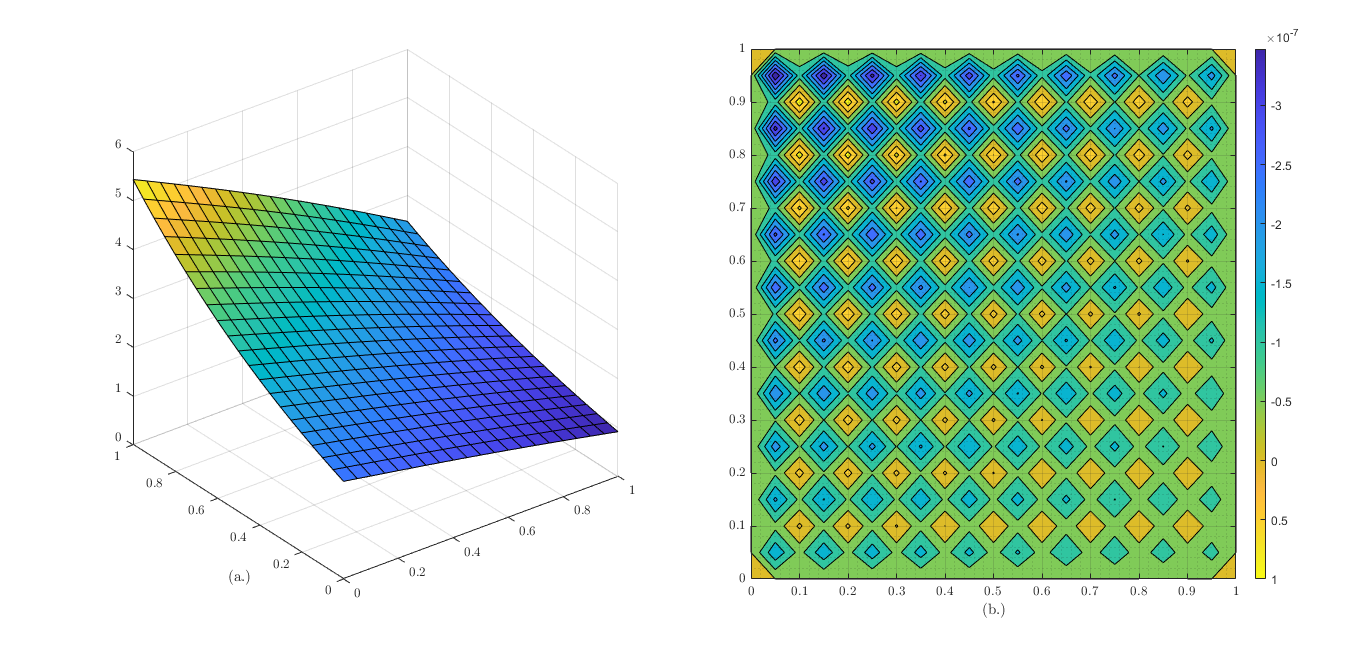
\includegraphics[scale = 0.60]{Images/poisson_comp.png}
    \caption[Approximate Solution to the Poisson Problem]{(a.) Approximate solution to the given BVP and (b.) the relative error in the analytical and the approximate solution.}
    \label{fig:Poisson_FEM}
\end{figure}
    
 The convergence of the approximate solution to the exact solution is investigated by plotting the $L^{2} error$ against
 increasing number of elements in the mesh for various Gauss quadrature points \footnote{The data for the solution with
 a singular element encompassing the domain has been skipped as it leads to a trivial solution for the case of a first
 order quardilateral element.}.

 \begin{figure}
    \centering
    \subfloat{\hspace*{-3.5cm}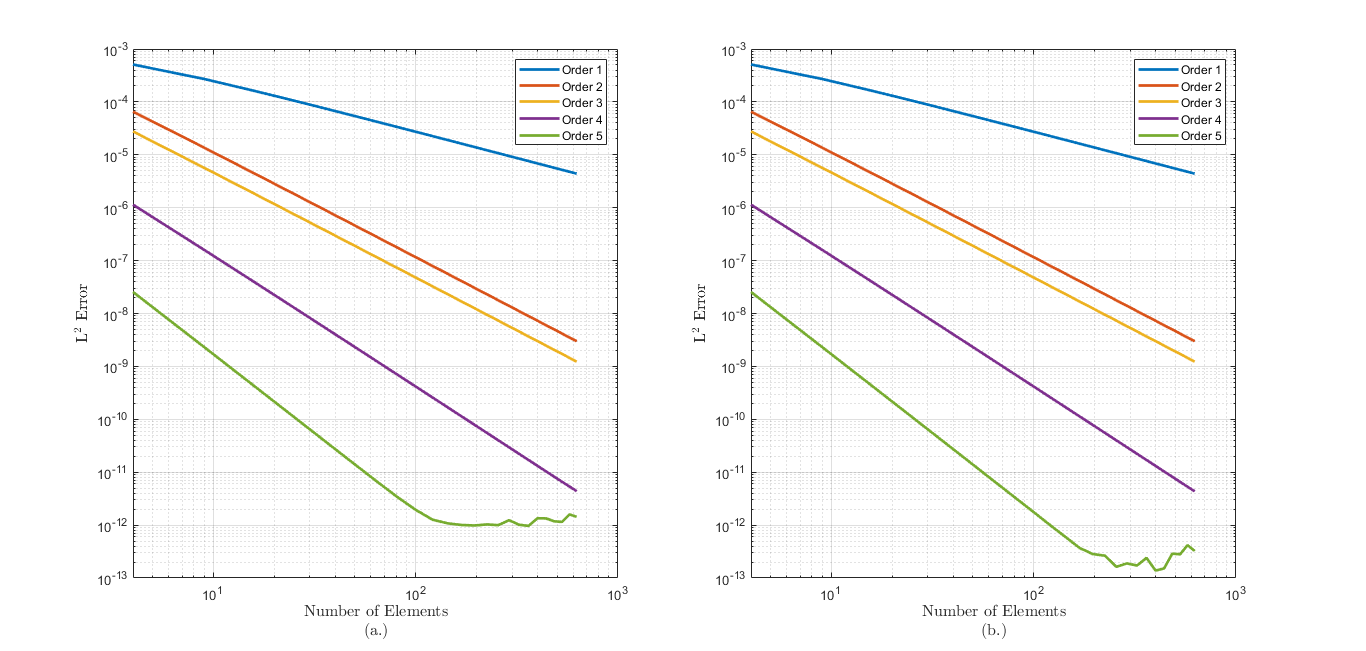
\includegraphics[scale = 0.60]{Images/conv68.png}} \\ %%\label{fig:a}} 
    \subfloat{\hspace*{-3.5cm}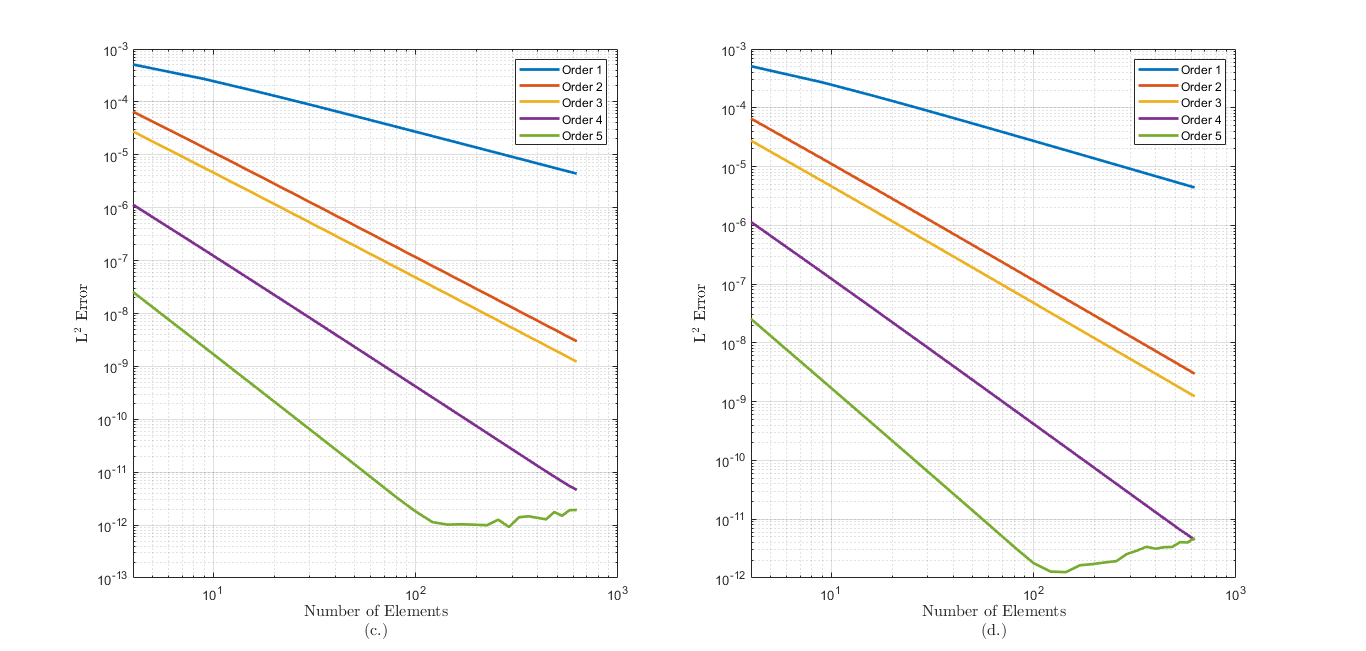
\includegraphics[scale = 0.60]{Images/conv1012.png}} %%\label{fig:b}}
    \caption[Convergence of the Approximate Solution]{Convergence of the approximate solution using various orders of approximating polynomial and (a.) 6, (b.) 8, (c.) 10, and (d.) 12 Gauss-Quadrature points.} %%\label{fig:AB}
  \end{figure}

In this section we developed the Finite Element framework for the solution of boundary value problems, investigated the
 validity of the resulting approximated solutions using \emph{a posteriori} error estimates, and tested if the approximated
 solution converges to the exact solution. This was done in order to lay the foundation for the development of a more complex
 framework in the next section in order to study the nonlinear behaviour of large deformations.

\afterpage{\blankpage}
% Chapter 1

\chapter{Nonlinear FEM Framework in Orthogonal Basis} % Main chapter title

\label{Chapter3} % For referencing the chapter elsewhere, use \ref{Chapter1} 

%----------------------------------------------------------------------------------------
%----------------------------------------------------------------------------------------

\section{Continuum Mechanics and Kinematical Relations} \label{sec:continuum_kinematics}

\begin{figure}  
    \centering
    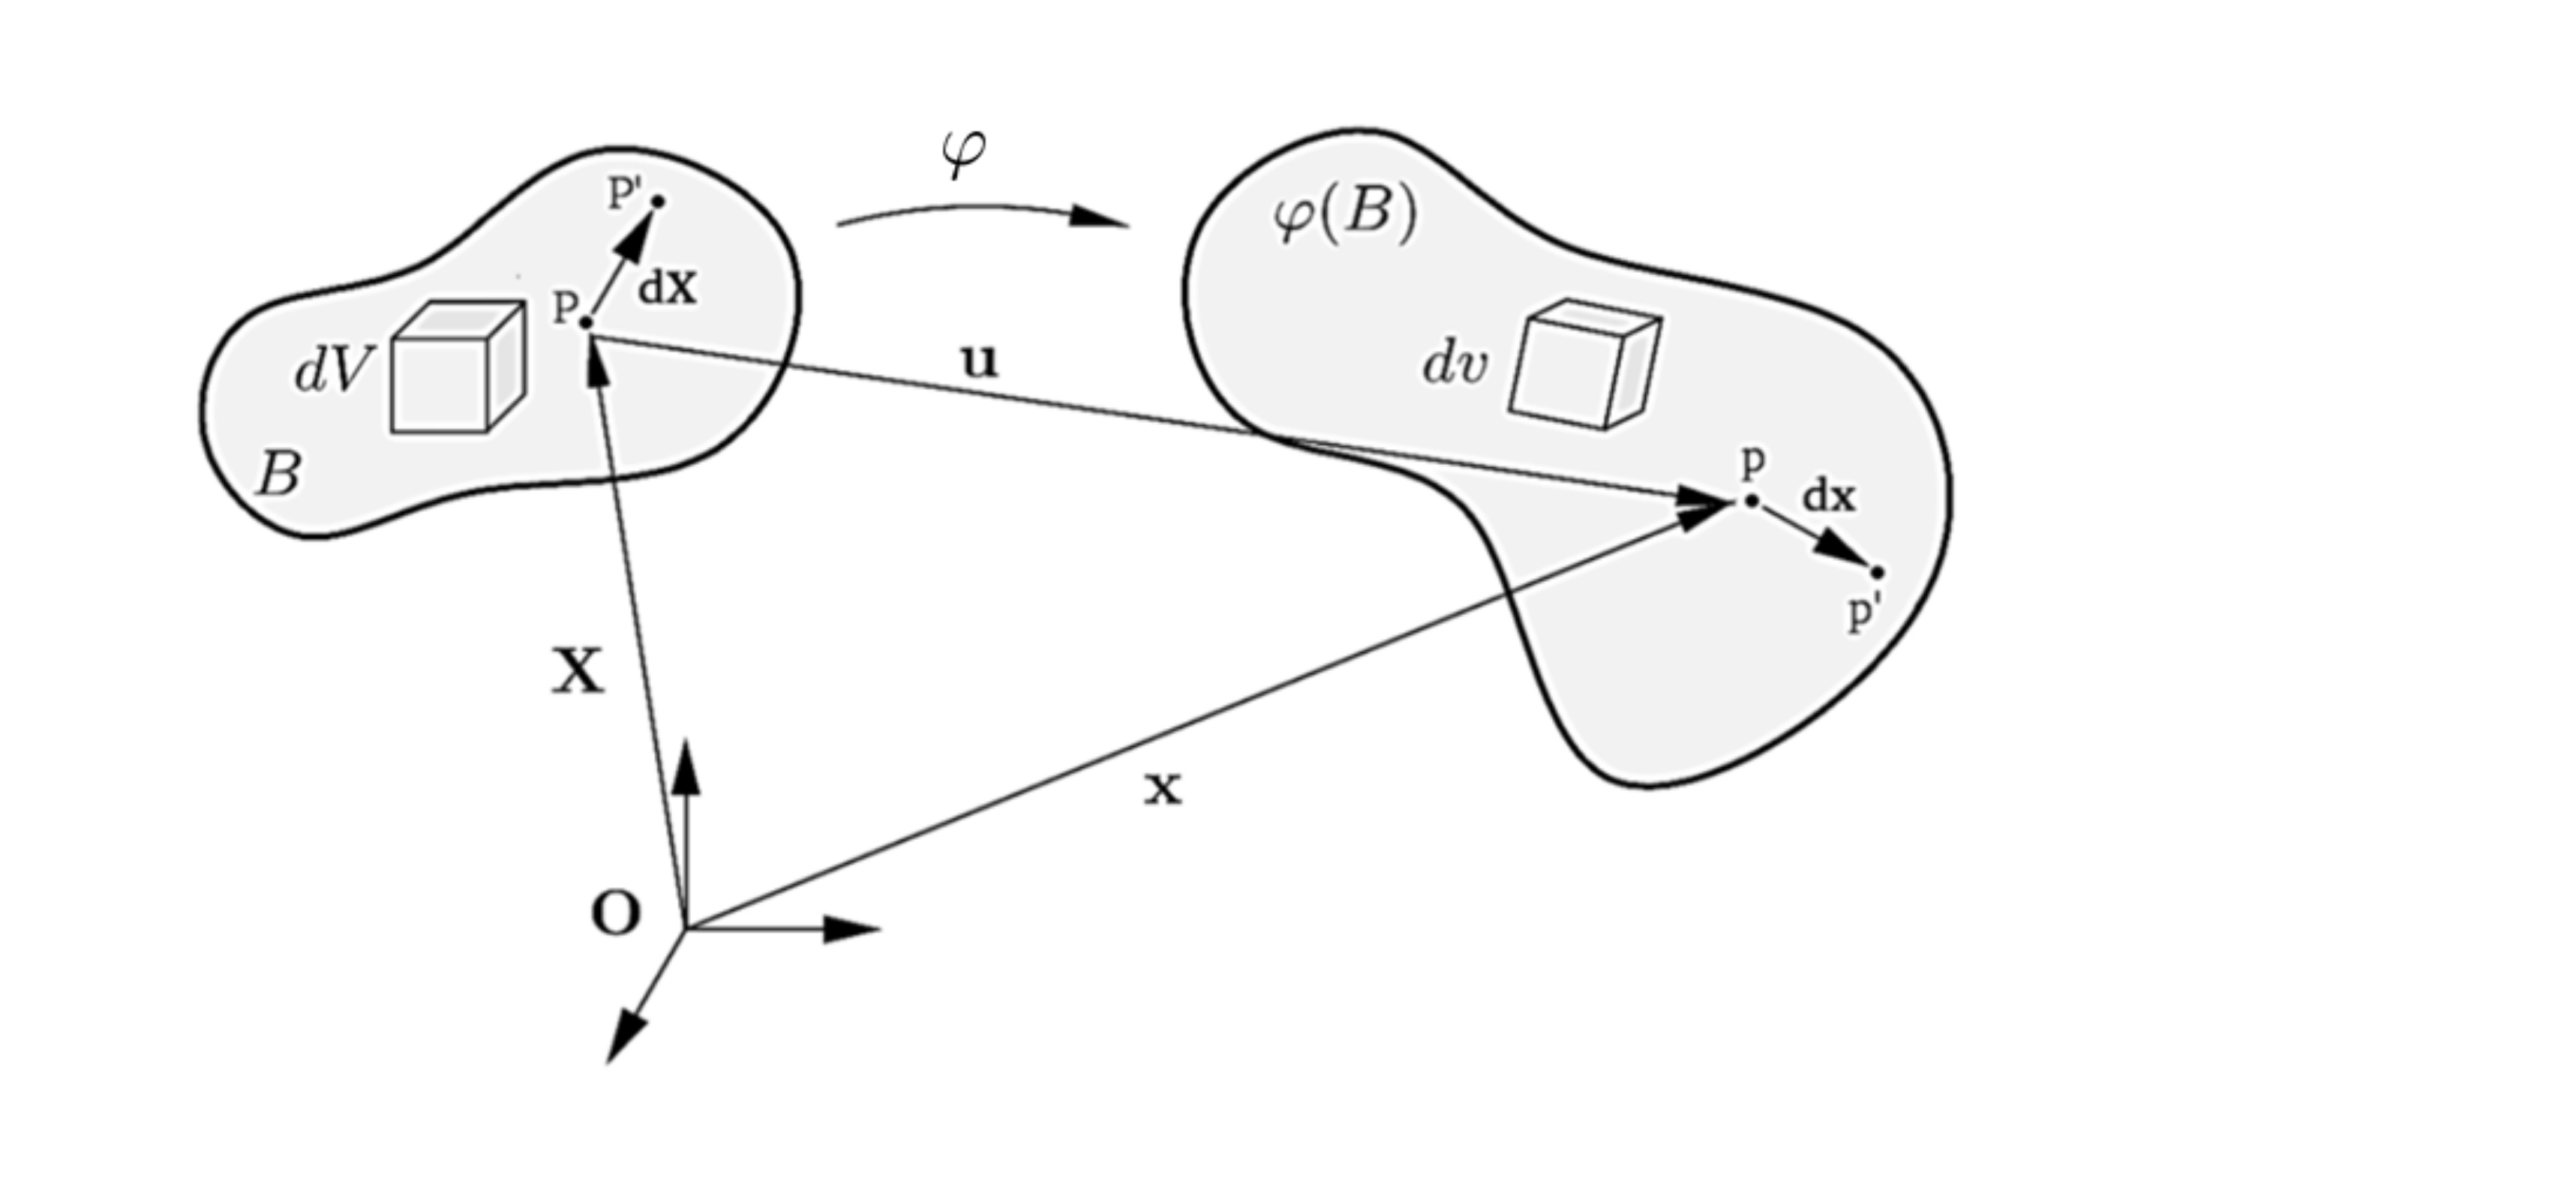
\includegraphics[scale = 0.60]{Images/ortho_map.png}
    \caption[Configuration and Motion of a Continuum Body in Orthogonal Basis]{Configuration and motion of a continuum body in orthogonal basis (Image Source: Institute of Applied Mechanics, RWTH Aachen).}
    \label{fig:km_config}
\end{figure}
According to continuum mechancis, a body $\mathcal{B}$ is defined as a manifold consisting of finite number of particles.
 This body $\mathcal{B}$ is also assumed to be a $\sigma-\text{finite measure space}$ - 
 this implies that each subset of $\mathcal{B}$ is associated with a non-negative measure, 
 which in this case would be the mass distribution.
 This manifold is assumed to be smooth, sufficiently differentiable, and the configuration of the particales at a given time
 can be mapped one-to-one onto Euclidean space, $\varphi: \mathcal{B} \rightarrow \mathbb{E}^{3}$, thus assigning a position vector to 
 each particle of the body in $\mathbb{E}^{3}$ \cite{truesdell2012,wriggers2008}. For simplicity, an orthogonal cartesian basis is assumed in this section as
 the formulation will be based on isoparametric interpolations - which rely on an orthogonal basis. A more general
 description using curvilinear coordinates is covered in Section \ref{sec:curvy_coords}. 
In order to ease the description of motion and deformation, it is convenient to assume a \emph{reference configuration}
 at an fixed time $t = t_{0}$. In this configuration, the body is assumed to be unloaded, undeformed, and unstressed.
 For an arbitrary point on the body $\mathrm{P}$ a position vector can be defined with respect to the origin of the basis,
\begin{equation}\label{ref_config_defition}
    \begin{cases}
        \boldsymbol{X} &= \boldsymbol{\varphi}(X, t_{0}),\\
        \boldsymbol{X} &= X^{i} \, \boldsymbol{E}_{i}\, , \, \, \text{where } {X}^{i}: {X}^{1}, {X}^{2}, {X}^{3} 
    \end{cases}
    \end{equation}
and $\boldsymbol{E}_{i}$ are unit vectors along the ${X}^{i}$ axes.

At any other time \emph{t} the configuration of the body will be referred to as the \emph{current configuration}.
 This mapping of the reference configuration into the current configuration is assumed to be so that all points in
 both configurations are mapped one-to-one. The position vector of the point $\mathrm{P}$
 that has now moved due to external forces to a position $\mathrm{p}$ can be defined as
\begin{equation} \label{curr_config_definition}
    \begin{cases}
        \boldsymbol{{x}} &= \boldsymbol{\varphi_{t}}(\boldsymbol{X}, t), \\
        \boldsymbol{{x}} &= {x}^{i} \, \boldsymbol{{e}}_{{i}}\, , \, \, \text{where } {x}^{i}: {x}^{1}, {x}^{2}, {x}^{3}.
    \end{cases}
\end{equation}
Similarly, $\boldsymbol{{e}}_{{i}}$ are the unit vectors
 along the ${x}^{i}$ axes.

Two consequences follow the assumption of a cartesian basis system. The dual basis to the unit vectors $\boldsymbol{{E}}_{{i}}$ and $\boldsymbol{{e}}_{{i}}$
 reduces to the original basis, thus making the position of the indices immaterial. Furthermore, as $\boldsymbol{E}$ and $\boldsymbol{e}$ are self adjoint,
 it can be shown that $\boldsymbol{{E}}_{{i}} = \boldsymbol{{E}}^{{i}} = \boldsymbol{{e}}_{{i}} = \boldsymbol{{e}}^{{i}}$, thus making the unit
 vectors and the position of the indices in both the configurations interchangeable without any effects to the maths involved.
The position vector of the point $\mathrm{p}$ relative to $\mathrm{P}$ is called the displacement vector $\boldsymbol{{u}}$ and can be defined as
\begin{equation} \label{displacement_vector}
    \boldsymbol{{u}} = \boldsymbol{{x}} - \boldsymbol{{X}} = {U}^{{i}} \boldsymbol{{E}}_{{i}} = {u}^{{i}} \boldsymbol{{e}}_{{i}}.
\end{equation}
In the reference configuration an infinitesimal vectorial line element between two points can be written as $\mathrm{d}\boldsymbol{X}$.
 Similarly, $\mathrm{d}\boldsymbol{x}$ can be defined as the infinitesimal vectorial line element between the corresponding points in the current configuration.
 The mapping from $\mathrm{d\boldsymbol{X}}$ to $\mathrm{d\boldsymbol{x}}$ can be used to study the deformation of the body. This
 mapping can be represented with the help of a second order tensor called the \emph{deformation gradient}.
 \begin{gather} \label{deformation_gradient}
    \mathrm{d}\boldsymbol{x} = \boldsymbol{{F}} \, \mathrm{d}\boldsymbol{X} \\
    \boldsymbol{{F}} := \mathrm{Grad} \, \boldsymbol{{x}} = \frac{\partial \boldsymbol{{x}}}{\partial \boldsymbol{{X}}^{{i}}} \otimes \boldsymbol{{e}}^{{i}} = \frac{\partial{x}^{i}}{\partial {X}^{{j}}} \, \boldsymbol{{e}}_{{i}} \otimes \boldsymbol{{e}}^{{j}} = {F}^{{i}}_{.j} \, \boldsymbol{e}_{i} \otimes \boldsymbol{e}^{j} 
\end{gather}
The deformation gradient further allows the transformation of differential quantities from the reference to the current configuration.
 A differential area element $\mathrm{d}\boldsymbol{a}$ in the current configuration can be written in terms of the area element $\mathrm{d}\boldsymbol{A}$ in the reference configuration
 using Nanson's formula,
 \begin{equation} \label{Nansons}
    \mathrm{d}\boldsymbol{a} = \mathbf{n} \,da = J \boldsymbol{F}^{-T} \boldsymbol{N} \,dA = J \boldsymbol{F}^{-T} \mathrm{d}\boldsymbol{A},
 \end{equation}
 where $\boldsymbol{n}$ and $\boldsymbol{N}$ are the normal vectors of the area elements $\mathrm{d}\boldsymbol{a}$ and $\mathrm{d}\boldsymbol{A}$ respectively, and $J$ is the determinant of the deformation gradient
 \begin{equation}\label{jacobian_deformation_gradient}
    J = \det\boldsymbol{F}.
 \end{equation}
 This also enables us to construct a relation between the differential volume elements,
 \begin{equation} \label{volume}
    dv = J\,dV.
 \end{equation}
The squares of the line elements $\mathbf{d}\boldsymbol{x}$ and $\mathbf{d}\boldsymbol{X}$ are related with the use of the right and left \emph{Cauchy-Green tensors} represented as $\boldsymbol{C}$ and
 $\boldsymbol{b}$ respectively, that are defined as,
\begin{align} \label{cauchy_green_tensors}
    \mathrm{d}\boldsymbol{x} \cdot \mathrm{d}\boldsymbol{x} &= \mathrm{d}\boldsymbol{X} \cdot \boldsymbol{C} \mathrm{d}\boldsymbol{X}, \text{ where } \boldsymbol{C} := \boldsymbol{F}^{T}\boldsymbol{F},\\
    \mathrm{d}\boldsymbol{X} \cdot \mathrm{d}\boldsymbol{X} &= \mathrm{d}\boldsymbol{x} \cdot \boldsymbol{b}^{-1} \mathrm{d}\boldsymbol{x}, \text{ where } \boldsymbol{b} := \boldsymbol{F} \boldsymbol{F}^{T},
\end{align}
which enables us to define the strain measures based on the difference between the squared lengths
 $\Vert\mathrm{d}\boldsymbol{x} \cdot \mathrm{d}\boldsymbol{x}\Vert^{2} - \Vert\mathrm{d}\boldsymbol{X} \cdot \mathrm{d}\boldsymbol{X}\Vert^{2} $, known as the \emph{Green-Lagrange strain tensor} and the \emph{Almansi strain tensor} respectively
\begin{align} \label{strain_measures}
    \boldsymbol{E} &:= \frac{1}{2} \left(\boldsymbol{C} - \boldsymbol{I}\right),\\
    \boldsymbol{e} &:= \frac{1}{2} \left(\boldsymbol{I} - \boldsymbol{b}^{-1}\right).
\end{align}
\section{Stress and Balance Equations}
On a body $\mathcal{B}$, the Cauchy stress vector $\mathbf{t}$ refers to a force per unit area of the deformed surface with a unit normal vector
\begin{equation} \label{traction_vector_definition}
    \mathbf{t} = \lim_{\Delta a \rightarrow 0} \frac{\mathbf{\Delta p}}{\Delta a}. 
\end{equation}
According to the \emph{Cauchy postulate}, the stress vector $\mathbf{t}$ is only dependent on the unit normal $\mathbf{n}$ and not on any other characteristic
 of the surface. This mapping between the stress vector and the unit normal can be represented with the help of a second order tensor called the \emph{Cauchy stress tensor}
 \begin{equation} \label{cauchy_stress_tensor}
    \mathbf{t} = \boldsymbol{\sigma} \mathbf{n}, \text{ where } \boldsymbol{\sigma} = \sigma^{ij} \mathbf{e}_{i} \otimes \mathbf{e}_{j}.
 \end{equation}

The fundamental relations of continuum mechanics are the balance relations.
 They are stated in the following briefly and without proof. The derivations can be found in \cite{wriggers2008} and \cite{itskov2020}.
\subsection{Balance of Mass}
For a closed system, the total mass is conserved i.e. over a given period of time, the change in mass ($\dot{m}$) is zero.
 This implies that the mass of the body in the reference configuration is equal to the 
 mass of the body in the current configuration.
\begin{align}\label{mass_balance}
    \dot{m} &= 0,\\
    \rho \, dv &= \rho_{0} \, dV,
\end{align}
where $\rho$ and $dv$ are the mass density and the volume of the body in the current configuration, and 
 $\rho_{0}$ and $dV$ are the density and volume of the body in the reference configuration.
\subsection{Balance of Linear Momentum}
The rate of change of linear momentum of a body is equal to the sum of the external forces acting on the body.
\begin{equation}\label{lin_momentum_balance}
    \begin{cases}
        \mathrm{div} \boldsymbol{\sigma} + \boldsymbol{f} = \rho \, \boldsymbol{\ddot{x}},\\
        \sigma ^{ij}||_{j} + f^{i} = \rho \, a^{i},
    \end{cases}  
\end{equation}
where $\boldsymbol{f}$ is the sum of forces acting on a body excluding inertia, $\boldsymbol{a} := \boldsymbol{\ddot{x}} = a^{i} \boldsymbol{e}_{i}$
 is the acceleration of a particle with the position vector $\boldsymbol{x}$.
The First Piola-Kirchhoff stress tensor can be used to represent the linear momentum balance in the reference configuration that can be written as
\begin{equation}\label{lin_momentum_balance_refconfig}
    \begin{cases}
        \mathrm{Div} \boldsymbol{{P}} + \boldsymbol{f}_{0} = \rho_{0} \, \boldsymbol{\ddot{x}},\\
        P^{ij}|_{j} + f_{0}^{i} = \rho_{0} \, a_{0}^{i}.\
    \end{cases}
\end{equation} 
In \eqref{lin_momentum_balance} and \eqref{lin_momentum_balance_refconfig}, the differential operators $(\bullet)|_{j}$
 and $(\bullet)||_{j}$ are the covariant derivatives in the current and the reference configurations respectively.
\subsection{Balance of Angular Momentum}
The rate of change of angular momentum of a body is equal to the resultant moment of the external forces acting on the body.
\begin{equation}\label{angular_momentum}
    \int_{\mathcal{B}} \rho(\boldsymbol{x}\, \times \boldsymbol{v}) = \int_{\mathcal{B}} \rho(\boldsymbol{x}\, \times \boldsymbol{b}) + \int_{\partial\mathcal{B}} (\boldsymbol{x}\, \times \boldsymbol{t}).
\end{equation}
This results in the local balance of angular momentum which simply requires the Cauchy stress tensor to be symmetric
\begin{align} \label{cauchy_stress_sym}
    \boldsymbol{\sigma} &= \boldsymbol{\sigma ^{T}},\\
    \sigma _{ij} &= \sigma _{ji}.
\end{align}
\subsection{Balance of Kinetic Energy}
An extension of \eqref{lin_momentum_balance}, is the balance of kinetic energy which states that the power of external forces $P$
 is equal to the sum of the stress power $W$ and the change in kinetic energy $\dot{K}$ of a body.
\begin{gather}\label{kin_energy}
    P = W + \dot{K},\\
    \int_{\mathcal{B}} \rho \,\boldsymbol{\overline{\mathrm{b}}} \cdot \boldsymbol{\mathrm{v}} \, dv + \int_{\partial \mathcal{B}} \boldsymbol{\mathrm{t}} \cdot \mathrm{\boldsymbol{v}} \, da =
    \int_{\mathcal{B}} \boldsymbol{\sigma} : \boldsymbol{\mathrm{d}} \,dv + \int_{\mathcal{B}} \frac{1}{2} \rho \mathrm{\boldsymbol{v}} \cdot \mathrm{\boldsymbol{v}} \, dv. \notag
\end{gather}
Represented by the Cauchy stress tensor, $\boldsymbol{\sigma}$, and the rate of deformation tensor, \textbf{d},
 the stress power can be decomposed further into heat production, $\mathcal{D}$ ad the stored energy density, $\Psi$, as follows
\begin{equation}\label{stress_power}
    W = \mathcal{D} + \int_{\mathcal{B}} \dot{\Psi}\,dV_{0}.
\end{equation} 
\subsection{Conservation of Energy}
The First Law of Thermodynamics states that the rate of change of the total energy $\dot{E}$ of a system is equal to the
 sum of the mechanical power of the external loads $P$ and the heat supplied $Q$ to the system.
\begin{gather}\label{first_thermo}
    \dot{E} = P + Q,\\
    \frac{\mathrm{d}}{\mathrm{dt}}\left[\int_{\mathcal{B}} \frac{1}{2} \rho \mathrm{\boldsymbol{v}} \cdot \mathrm{\boldsymbol{v}} \, dv + \int_{\mathcal{B}} \rho u \, dv\right] = 
    \int_{\mathcal{B}} \rho \,\boldsymbol{\overline{\mathrm{b}}} \cdot \boldsymbol{\mathrm{v}} \, dv + \int_{\partial \mathcal{B}} \boldsymbol{\mathrm{t}} \cdot \mathrm{\boldsymbol{v}} \, da - \int_{\partial \mathcal{B}} \boldsymbol{\mathrm{q}} \cdot \boldsymbol{\mathrm{n}} \, da + \int_{\mathcal{B}} \rho \, r \,dv, \notag
\end{gather}
where \textbf{q} and \textbf{n} are the heat flux vector and the surface normal respectively, and \emph{r} is the distributer inner heat source.
\section{Constitutive Relations}
Constitutive relations are the properties of the material under investigation. They characterise the material response of a body and
 are necessary to complete the system of differential equations for the solution of boundary value problems \cite{itskov2020}. Materials in the real world can exhibit incredibly diverse behaviours making it necessary for the constitutive relations to
 have a degree of approximation involved in their formulation. However, the relations must agree with the observed experimental behaviours. All constitutive relations must satisfy the 
 second law of thermodynamics and three general principles that are known as \emph{Noll's axioms}.
 These are the \emph{principle of determinism}, which states that the stress in a particular point can be determined by 
 the stress history at that point; the \emph{principle of local action},
 that states that the stress at a particular point is affected by the motion of the particles in
 immediate neighbourhood of that point; and the \emph{principle of material objectivity}, which states that the choice of coordinate
 system should not affect the material properties. 
Hyperelastic materials can be characterised by having zero heat dissipation. Thus the stress power \eqref{stress_power}
 reduces to
 \begin{equation}\label{hyper_stress_power}
    W = \int_{\mathcal{B}} \dot{\Psi}\,dV_{0}.
 \end{equation}
Comparing equations \eqref{kin_energy} and \eqref{hyper_stress_power}, according to \cite{itskov2020},
 \begin{gather}\label{S_is_Psi}
    \dot{\Psi} = \mathrm{J} \boldsymbol{\sigma} : \mathrm{\boldsymbol{d}} = \mathrm{\boldsymbol{S}} : \frac{1}{2}\mathrm{\boldsymbol{\dot{C}}} = 2 \frac{\partial \Psi}{\partial \mathrm{\boldsymbol{C}}} : \frac{1}{2} \mathrm{\boldsymbol{\dot{C}}}, \notag\\
    \therefore \, \mathrm{\boldsymbol{S}}  = 2 \frac{\partial \Psi}{\partial \mathrm{\boldsymbol{C}}}.
\end{gather}
Neo-Hookean materials are examples of hyperelastic materials. The model can be used to approximate the behaviour of
 rubber like materials fairly accurately for strains upto 20\% \cite{gent2001}. Given a Neo-Hookean material model defined as,
\begin{equation} \label{neo_hookean_definition}
{\boldsymbol{\sigma} = \frac{\mu}{J}\left(\boldsymbol{b}-\boldsymbol{I}\right) + \frac{\Lambda}{J}\ln{J}\boldsymbol{I}}
\end{equation}
The expression for the compliance matrix in the reference configuration can be written as

\begin{equation} \label{compliance_definition}
    {\mathbb{C} = 4\frac{\partial^2 \Psi}{\partial\boldsymbol{C}\partial\boldsymbol{C}} = 2\frac{\partial\boldsymbol{S}}{\partial\boldsymbol{C}}}
\end{equation}
 where \textbf{S} is the second Piola-Kirchhoff stress tensor which is defined as,
\begin{equation}\label{eq:19}
    {\boldsymbol{S} = J \boldsymbol{F^{-1} \sigma F^{-T}}}
\end{equation}
The given material model can be written using the Second Piola Kirchhoff Stress Tensor.
\begin{equation}\label{neo_hookean_S}
    {\boldsymbol{S} = \mu\left(\boldsymbol{I} - \boldsymbol{C^{-1}}\right) + \Lambda\ln{J}\boldsymbol{C^{-1}}}
\end{equation}
The compliance matrix is a fourth order tensor and using \eqref{neo_hookean_S} and \eqref{compliance_definition} can be written in the indicial form as follows
\begin{equation}\label{compliance_matrix_reference}
    \mathbb{C}^{i.a.}_{.j.b} = 2\left(-\mu + \Lambda\ln{J}\right)\left(C^{-1}\right)^i_{.a} \left(C^{-1}\right)^b_{.j} + \Lambda \left(C^{-1}\right)^i_{.j} \left(C^{-1}\right)^a_{.b}.
\end{equation}
Applying push-forward to \eqref{compliance_matrix_reference} to transform $\mathbb{C}$ to the current configuration,
\begin{equation} \label{compliance_matrix_current}
    \mathbbmss{c}^{i.a.}_{.j.b} = 2\left(-\mu + \Lambda\ln{J}\right) \delta^i_{.a} \delta^b_{.j} + \frac{\Lambda}{2} \delta^i_{.j} \delta^a_{.b}.
\end{equation}

\section{Weak Form}
Using the strong form of the linear momentum balance, \eqref{lin_momentum_balance},
 the weak form can be derived using a test function as described in Section \ref{sec:poisson_weak_form} and the contributions can be 
 separated into \emph{internal virtual work} and \emph{external virtual work}. A derivation of the weak form using
 general curvilinear coordinates can be found in Section \ref{sec:curvy_weak_form}, which can be reduced to obtain the following 
\begin{equation} \label{weak_form_beam}
    \underbrace{\int_{\mathcal{B}} \mathrm{grad}(\boldsymbol{w}) : \boldsymbol{\sigma} \,dv}_{\text{internal virtual work}} - 
        \underbrace{\int_{\mathcal{B}} \boldsymbol{w}\cdot \rho \overline{\boldsymbol{b}} \,dv - \int_{\partial_{t}\mathcal{B}} \boldsymbol{w} \cdot \overline{\boldsymbol{t}} \,da}_{\text{external virtual work}} = 0
\end{equation}
where the contributions of the internal virtual work and external virtual work can be defined as $G_{int}$ and $G_{ext}$ respectively.

\section{Discretisation} \label{sec:nonlinear_discretisation}
The reference configuration $\mathcal{S}_{0}$ is discretised into a set of finite elements, $\Omega_{0}^{e}$ that are defined by nodal points
 $\boldsymbol{X}$. Thus, the current configuration is composed by finite elements $\Omega^{e}$ with nodal points $\boldsymbol{x}$
 that are related to $\boldsymbol{X}_{I}$ through relations described in \ref{sec:continuum_kinematics}. 

After the discretisation of the domain into finite elements, the shape functions can be used to discretise the nodal variables
 in the reference and current configurations $\boldsymbol{X}$ and $\boldsymbol{x}$, the primary field variables $\boldsymbol{u}$,
 and the test functions $\boldsymbol{w}$ within each finite element can be discretised using the shape functions according to the isoparametric concept
 as described in Section \ref{sec:isoparametric_theory}. 
 Given a finite element domain, $\Omega$, and shape functions, $\boldsymbol{N}^{e}$,
 \begin{align} \label{nodal_discretisations}
    \boldsymbol{X} &\approx \boldsymbol{X}^{h} = \sum^{n_{en}}_{k=1} N^{e}_{k} X^{e}_{n} = \mathbf{N}^{e}\mathbf{X}^{e},\\
    \boldsymbol{x} &\approx \boldsymbol{x}^{h} = \sum^{n_{en}}_{k=1} N^{e}_{k} x^{e}_{n} = \mathbf{N}^{e}\mathbf{x}^{e},\\
    \boldsymbol{u} &\approx \boldsymbol{u}^{h} = \sum^{n_{en}}_{k=1} N^{e}_{k} u^{e}_{n} = \mathbf{N}^{e}\mathbf{u}^{e},\\
    \boldsymbol{w} &\approx \boldsymbol{w}^{h} = \sum^{n_{en}}_{k=1} N^{e}_{k} w^{e}_{n} = \mathbf{N}^{e}\mathbf{w}^{e},
 \end{align}
where the summation is carried over the $n_{en}$ nodes of the element. 
Using the above given definitions, and the weak form of the momentum balance \eqref{weak_form_beam}, the discretised form of the weak form
 in its internal virtual work contributions as summed over $n_{el}$ elements can be given as,
\begin{align} \label{discretised_g_int}
    G_{\text{int}} \approx G^{e}_{\text{int}} = \sum^{n_{el}}_{e=1} G^{e}_{\text{int}}, \,\,\text{where } \, \, G^{e}_{\text{int}} &= \int_{\Omega^{e}} \mathrm{grad}(\boldsymbol{w}) : \boldsymbol{\sigma} \,dv \notag\\
    \text{and }\,\, G^{e}_{int} &= \mathbf{w}^{T}_{e} \int_{\Omega^{e}}{\mathbf{B}^{T}_{e}} \boldsymbol{\sigma}_{v} \,dv =: \mathbf{w}^{T}_{e} \mathbf{f}^{e}_{\text{int}}
\end{align}
As the Cauchy stress tensor is symmetric in this framework, to ease computation we can take use of the Voigt notation. 
 Thus, $\boldsymbol{\sigma}_{v}$ is the stress tensor written in the Voigt notation,
\begin{equation}
    \boldsymbol{\sigma}_{v} = \begin{Bmatrix}
        \sigma_{11}\\
        \sigma_{22}\\
        \sigma_{33}\\
        \sigma_{23}\\
        \sigma_{31}\\
        \sigma_{12}
    \end{Bmatrix}
\end{equation}
And the matrix $\mathbf{B}_{e}$ is defined as,
\begin{align}
    \mathbf{B}_{e} &:= [\mathbf{B_{1}}, \mathbf{B_{2}}, \dots, \mathbf{B_{n}}], \notag\\
    \notag \\ 
    \mathbf{B}_{A} &= \begin{bmatrix}
        N_{A,x_{1}} & 0 & 0 \\
        0 & N_{A,x_{2}} & 0 \\
        0 & 0 & N_{A,x_{3}} \\
        0 & N_{A,x_{3}} & N_{A,x_{2}} \\
        N_{A,x_{3}} & 0 & N_{A,x_{1}} \\
        N_{A,x_{2}} & N_{A,x_{1}} & 0 \\
    \end{bmatrix}
\end{align}
%
Similarly, the external virtual work can be discretised,
\begin{align} \label{discretised_g_ext}
    G_{\text{ext}} \approx G^{e}_{\text{ext}} &= \sum^{n_{el}}_{e=1} G^{e}_{\text{ext}}, \notag \\
    &\text{where, }\,\, G^{e}_{\text{ext}} = \mathbf{w}^{T}_{e} \left[
    \int_{\Omega^{e}} \mathbf{N}^{T} \rho \overline{\boldsymbol{b}} \,dv + \int_{\Gamma^{e}} \mathbf{N}^{T} \overline{\boldsymbol{t}} \,da \right] =: \mathbf{w}^{T}_{e}\mathbf{f}^{e}_{\text{ext}}
\end{align}
%
Assembly of these force vectors, $\boldsymbol{\mathrm{f}}^{\mathrm{e}}_{\text{int}}$ and $\boldsymbol{\mathrm{f}}^{\mathrm{e}}_{\text{ext}}$, based on the element connectivity results in the discretised weak form,
 \begin{equation} \label{discretised_system_eq}
    \mathbf{w}^{T}[\mathbf{f}_{\text{int}} - \mathbf{f}_{\text{ext}}] = \boldsymbol{0}.
 \end{equation}

\section{Newton Raphson Method and Linearisation} \label{sec:newton_raphson_lin}
The Newton-Raphson method is an iterative method that can be used to approximate the roots of a nonlinear system of equations. 
 The algorithm subdivides a nonlinear system into linearised sub-problems and arrives at the global solution through the sequential
 solution of the sub-problems.
A given system of nonlinear equations, 
\begin{equation}
    \boldsymbol{f}(\boldsymbol{u}) = \boldsymbol{0},
\end{equation}
can be linearised using the Taylor series expansion as,
\begin{equation} \label{taylor}
    \boldsymbol{f}(\boldsymbol{u}+ \Delta \boldsymbol{u}) = \boldsymbol{f}(\boldsymbol{u}) + D \boldsymbol{f}(\boldsymbol{u}) \cdot \Delta \boldsymbol{u},
\end{equation}
after having ignored the higher order terms. In \eqref{taylor}, $D \boldsymbol{f}(\boldsymbol{u})$ is the directional derivative of
 $\boldsymbol{f}$ at $\boldsymbol{u}$. 
$D \boldsymbol{f}(\boldsymbol{u})$ can be written using the general $G\hat{a}teaux$ derivative \cite{sauer2016}. However, if $D \boldsymbol{f}(\boldsymbol{u})$ is linear
 in $\Delta \boldsymbol{u}$, it can be written using the $Frech\acute{e}t$ differential of $\boldsymbol{f}$ at $\boldsymbol{u}$ as,
 \begin{equation} \label{frechet}
    D \boldsymbol{f}(\boldsymbol{u}) := \boldsymbol{f'}\left(\boldsymbol{u}\right) \cdot \Delta \boldsymbol{u}, \text{ where, } f'(u)_{ij} = \frac{\partial f_{i}}{\partial u^{j}} (u).
 \end{equation}
In \eqref{frechet}, $\boldsymbol{f'}\left(\boldsymbol{u}\right)$ can be called the Jacobian or the tangent matrix. 

Since the test functions in \eqref{discretised_system_eq} are arbitrary, the system of equations reduce to 
\begin{equation} \label{we_start_NR}
    \mathbf{f} = \mathbf{f}_{\text{int}} - \mathbf{f}_{\text{ext}} = \boldsymbol{0}.
\end{equation}
To be able to use the Newton method to solve \eqref{we_start_NR}, the tangent matrix related to $\boldsymbol{G}_{\text{int}}$ needs to be calculated.
 Linearising $\boldsymbol{G}_{\text{int}}$ at the element level,
\begin{equation} \label{lin_Gint}
    D \boldsymbol{G}^{e}_{int} (\mathbf{u}, \Delta \mathbf{u}) \approx \mathbf{w}^{T}_{e} \int_{\Omega^{e}_{0}} \mathbf{N}^{T}_{,i} \sigma_{ij} \mathbf{N}_{,j} \,dv \,\Delta \mathbf{u}_{e}
        + \mathbf{w}^{T}_{e} \int_{\Omega^{e}_{0}} \mathbf{B}^{T} \mathbbmss{c}_{v} \mathbf{B} \,dv \,\Delta \mathbf{u}_{e}
\end{equation}
where 
\begin{equation}
    \mathbf{N}_{,i} = \frac{\partial \mathbf{N}}{\partial x^{i}}
\end{equation}
and $\mathbbmss{c}_{v}$ is the compliance matrix as derived in equation \eqref{compliance_matrix_current} written in the Voigt notation.

\section{Numerical Examples}
The validitation of the nonlinear Finite Element framework is done by considering two examples of a clamped beam
 with a prescribed displacement and a prescribed load at the unclamped end respectively. The length (normalised as $\frac{\mathrm{L}}{\mathrm{L}_0}$) and height (normalised as $\frac{\mathrm{H}}{\mathrm{H}_0}$) of the beam
 are taken to be 20 and 1 unit respectively and plane strain conditions are assumed. The beam is meshed with
 standard quadrilateral Lagrangian elements and the mesh can be refined with decreasing the element size or increasing the
 order of the approximation polynomial. The nodes on the clamped end of the beam are constrained in the x-direction. Additionally,
 the node on the clamped end that lies on the neutral axis of the beam is constrained in the y-direction. In the case of a prescribed displacement, the node lying on the neutral axis at the unclamped end is additionally assigned the prescribed displacement.
 No such constraint is applied to the aforementioned node in the case of the load driven boundary conditions. Both examples are
 utilise numerical integration as described in Section \ref{sec:quadrature} and the system of equations are solved using the Newton method.
Figures \ref{fig:beam_fe_disp} and \ref{fig:beam_fe_force} on the next page depict the deformation of the beam at various stages of deformation with the normal stress in the y-direction shown through the elements
 for the prescribed displacement and load conditions respectively.

In this section we developed a Finite Element framework to study large deformations and considered a numerical example for validation.
 The main aim of this framework was to serve as a halfway point between the simple Finite Element framework for the solution of boundary
 value problems and the development of a framework applicable to thin structures in curvilinear coordinates. Thus, a relatively
 simple numerical example was considered as the purpose was to test the functionality of the developed sub-functions for the
 manipulation of kinematical quantities, application of boundary conditions, and the solution of the nonlinear system of equations. The
 next section extends this framework to curvilinear coordinates. 

%\begin{figure} [h]
    %\hspace{\fill}
%    \centering
%    \begin{subfigure}[h]{0.48\textwidth}
%        %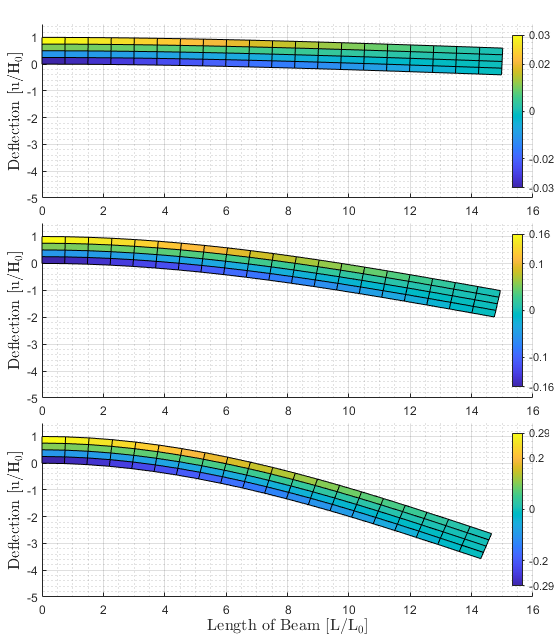
\includegraphics[height = 0.6\textheight, width = 0.5\paperwidth]{Images/beam_disp.png}
%        \hspace*{-2.9cm}
%        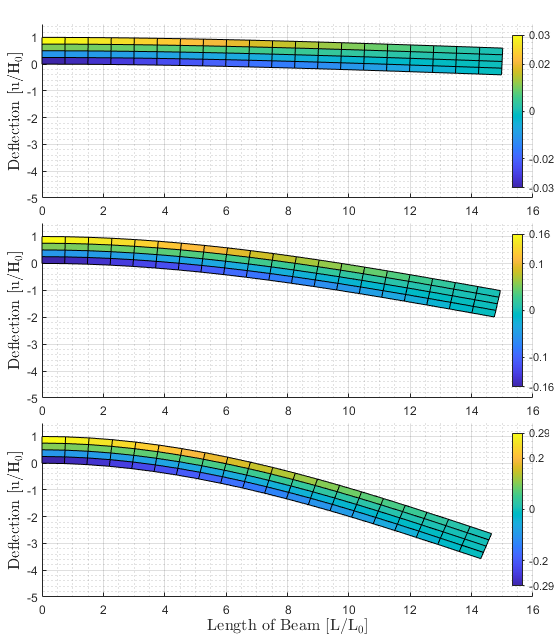
\includegraphics[scale = 0.7]{Images/beam_disp.png}
%        %\hspace{3.3cm}
%        \caption{Displacement driven boundary conditions}
%        \label{fig:beam_fe_disp}
%    \end{subfigure}
%    \hfill
%%    \begin{subfigure}[h]{0.48\textwidth} 
%        %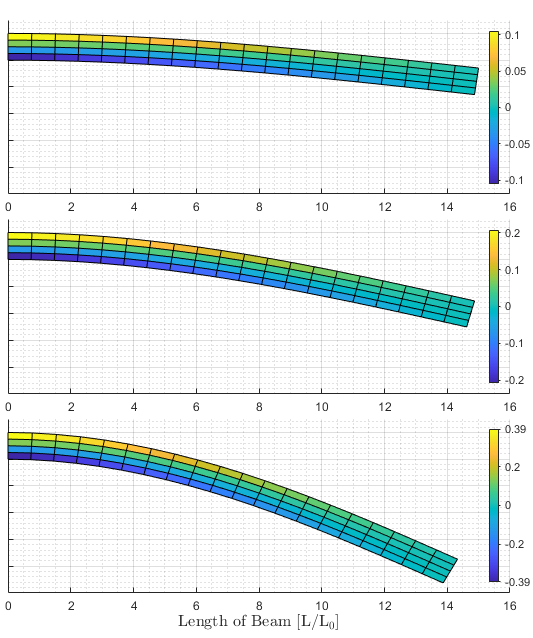
\includegraphics[height = 0.6\textheight, width = 0.5\paperwidth]{Images/beam_force.png}
%        %\hspace{0.25cm}
%        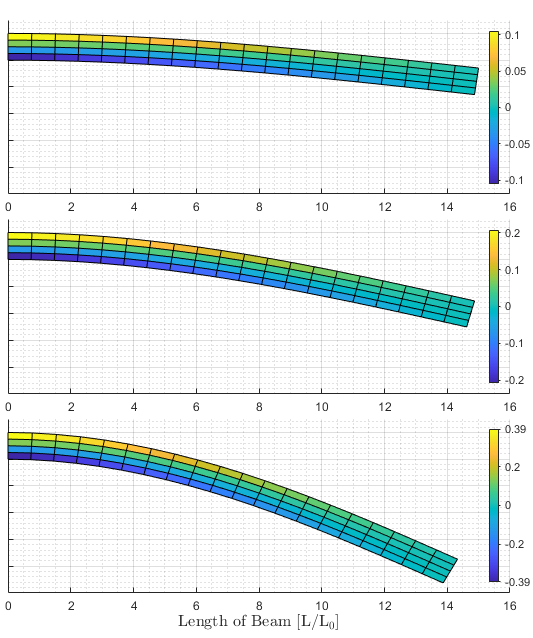
\includegraphics[scale = 0.7]{Images/beam_force.png}
%        %\captionsetup[subfigure]{oneside,margin={2cm,0cm}}
%        \caption{Force driven boundary conditions}
%        \label{fig:beam_fe_force}
%    \end{subfigure}
%    %\hspace*{\fill}
    
%    \caption{Numerical analysis of cantilever beam under various boundary conditions}
%    \label{fig:beam_fem}
%\end{figure}

\begin{figure}[h]
    \centering
    \begin{subfigure}{0.48\textwidth}
        \hspace*{-3cm}    
        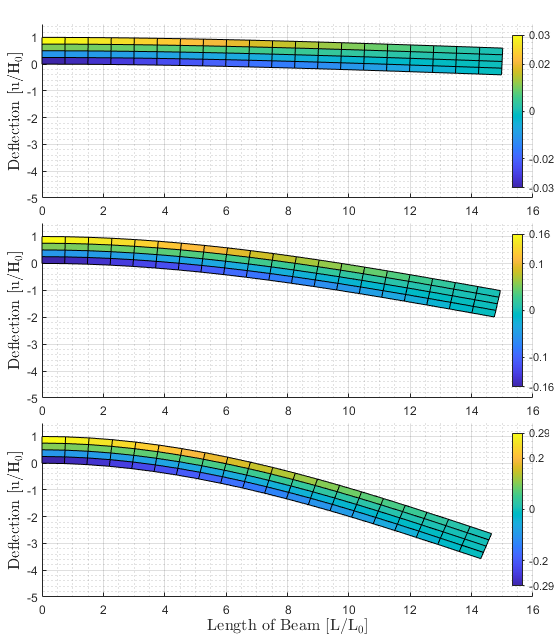
\includegraphics[scale = 0.70]{Images/beam_disp.png}
        \caption{Displacement driven boundary conditions}
        \label{fig:beam_fe_disp}
    \end{subfigure}
    \hfill
    \begin{subfigure}{0.48\textwidth}
        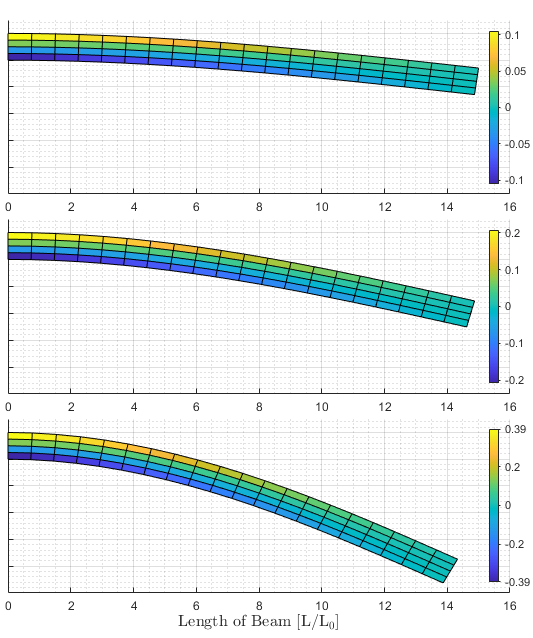
\includegraphics[scale=0.70]{Images/beam_force.png}
        \caption{Force driven boundary conditions}
        \label{fig:beam_fe_force}
    \end{subfigure}
    \caption[Numerical Analysis of Cantilever Beam]{Numerical analysis of cantilever beam under various boundary conditions}
    \label{fig:beam_fem}
\end{figure}
% Chapter 1

\chapter{Nonlinear FEM Framework in Curvilinear Basis} % Main chapter title

\label{Chapter4} % For referencing the chapter elsewhere, use \ref{Chapter1} 

%----------------------------------------------------------------------------------------

\section{Curvilinear Coordinates} \label{sec:curvy_coords}
Extending the continuum mechanics formulation to the formulation of shells,
 it becomes impossible to describe them using an orthogonal basis system for obvious reasons.
 Thus it is necessary to use a curvilinear coordinate system to account for the bent surface.
 Although shell model are often formulated using local cartesian coordinate systems as the
 classical relations described in the previous section can be extended to account for shells.
 However, the formulation under investigation feels unnecessary to make this detour and the relevant
 mathematics is described using curvilinear coordinates.
 \begin{figure}  
    \centering
    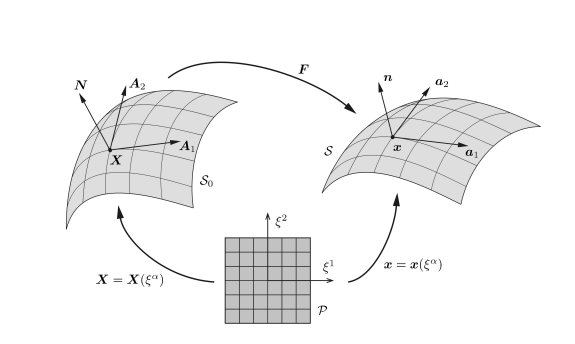
\includegraphics[scale = 0.60]{Images/curvilinear_map.png}
    \caption[Configuration and Motion of a Continuum Surface in Curvilinear Coordinates]{Configuration and motion of a continuum surface in curvilinear coordinates (Image Source: \cite{sauer2014}).}
    \label{fig:curvi_config}
\end{figure}
The membrane surface, denoted $\mathcal{S}$, is fully characterised by 
 the parametric description,
 \begin{equation} \label{parametric_definition}
    \boldsymbol{x} = \boldsymbol{x}(\xi^{1}, \xi^{2}) \, .
 \end{equation}
This is the mappinng of the point $(\xi^{1}, \xi^{2})$ in the parameter domain $\mathcal{P}$
 to the material point $\boldsymbol{x} \in \mathcal{S}$.
According to the non-standard tensor notation used in continuum mechanics,
 Greek indices take on the values 1 and 2 on the surface. And as in the previous section,
 lower case Latin indices take the values 1, 2, and 3, in Euclidean space and summation is
 implied on repeated indices.
The tangent vectors that form the basis at a coordinate $\xi^{\alpha}$ at point $\boldsymbol{x} \in \mathcal{S}$ are
 given by,
 \begin{equation}\label{tangent_parametric}
    \boldsymbol{a}_{\alpha} = \frac{\partial \boldsymbol{x}}{\partial \xi^{\alpha}}, \,\,\, \alpha = 1, 2
 \end{equation}
In general, they are not orthonomal. This basis is thus characterised by the \emph{first fundamental form} of the surface known as the covariant metric tensor,
\begin{equation}\label{metric_def}
    a_{\alpha \beta} := \boldsymbol{a}_{\alpha} \cdot \boldsymbol{a}_{\beta}.
\end{equation}
In case of an orthonormal basis system, the covariant metric tensor reduces to the identity tensor. The contravariant components of the metric tensor can be obtained by its inversion as
\begin{equation}\label{contravar_metric_def}
    [a^{\alpha \beta}] := [a_{\alpha \beta}]^{-1}.
\end{equation}
This enables the construction of a dual basis - the contra-variant counterparts of the covariant base vectors, $\boldsymbol{a}_{\alpha}$,
\begin{align}\label{contravar_def}
    \boldsymbol{a}^{\alpha} &:= a^{\alpha \beta} \boldsymbol{a}_{\beta},\\
    \boldsymbol{a}^{\alpha} &\cdot \boldsymbol{a}^{\beta} = a^{\alpha \beta},\\
    \boldsymbol{a}_{\alpha} &\cdot \boldsymbol{a}^{\beta} = \delta^{\beta}_{\alpha},
\end{align}
where $\delta^{\beta}_{\alpha}$ is the Kronecker delta.
%
The unit normal at a point $\boldsymbol{x} \in \mathcal{S}$ is defined by,
\begin{equation}\label{normal}
    \boldsymbol{n} = \frac{\boldsymbol{a}_{1} \times \boldsymbol{a}_{2}}{\| \boldsymbol{a}_{1} \times \boldsymbol{a}_{2} \|}
    = \frac{\boldsymbol{a}_{1} \times \boldsymbol{a}_{2}}{\sqrt{\det a_{\alpha \beta}}}.
\end{equation}

Any vector, $\boldsymbol{v}$ on $\mathcal{S}$ can thus be decomposed using the covariant or the contravariant basis,
\begin{equation}
    \boldsymbol{v} = v^{\alpha} \boldsymbol{a}_{\alpha} + v_{\mathrm{n}}\boldsymbol{n} = v_{\alpha} \boldsymbol{a}^{\alpha} + v_{\mathrm{n}}\boldsymbol{n},
\end{equation}
 where $v_{\alpha}$ and $v^{\alpha}$ denote the covariant and the contravariant components of the vector respectively.
The derivative and the co-variant derivative of the tangent vectors, $\boldsymbol{a}_{\alpha}$, can be defined as,
\begin{align}\label{tangent_derivatives}
    \boldsymbol{a}_{\alpha , \beta} &= \frac{\partial \boldsymbol{a}_{\alpha}}{\partial \xi^{\beta}},\\
    \boldsymbol{a}_{\alpha ; \beta} := \boldsymbol{a}_{\alpha , \beta} - &(\boldsymbol{a}_{\alpha , \beta} \cdot \boldsymbol{a}^{\gamma}) \boldsymbol{a}_{\gamma} = \boldsymbol{a}_{\alpha , \beta} - \Gamma^{\gamma}_{\alpha \beta} \boldsymbol{a}_{\gamma},
\end{align}
where $\Gamma^{\gamma}_{\alpha \beta}$ are the Christoffel symbols of the second kind.
Defining the identity tensor on the surface, $\mathcal{S}$,
\begin{equation}\label{surface_identity}
    \boldsymbol{1} = \boldsymbol{a}_{\alpha} \otimes \boldsymbol{a}^{\alpha} = \boldsymbol{a}^{\alpha} \otimes \boldsymbol{a}_{\alpha} = \boldsymbol{\tilde{1}} - \boldsymbol{n} \otimes \boldsymbol{n}, 
\end{equation}
where $\boldsymbol{\tilde{1}}$ is the usual identity tensor in $\mathbb{R}^{3}$, two results can be derived.
\begin{equation}\label{con_tgnt}
    \boldsymbol{a}_{\alpha ; \beta} = (\boldsymbol{n} \otimes \boldsymbol{n}) \boldsymbol{a}_{\alpha,\beta}.
\end{equation}
The \emph{second fundamental form} of the surface relates the change in the direction of the normal vector to the surface as the parametric coordinates are varied.
This is known as the curvature tensor with covariant components \footnote{The proofs to \eqref{con_tgnt} and \eqref{curvature_tensor_def} can be found in the appendix, \eqref{appendices:cov_tangent_derivative} and \eqref{appendices:curvature_tensor_derivation}.}
 $\boldsymbol{b} = b_{\alpha \beta} \boldsymbol{a}^{\alpha} \otimes \boldsymbol{a}^{\beta}$, where
\begin{equation} \label{curvature_tensor_def}
    b_{\alpha \beta} := \boldsymbol{n} \cdot \boldsymbol{a}_{\alpha ; \beta} = \boldsymbol{n} \cdot \boldsymbol{a}_{\alpha,\beta}.
\end{equation}
\section{Kinematics}
%---------------------------------------------------------------------------------
As defined in Section \ref{sec:continuum_kinematics}, to consider the deformation of the membrane surface, we distinguish between the reference configuration,
 $\mathcal{S}_{0}$, and the current configuration, $\mathcal{S}$. To describe quantities on $\mathcal{S}$,
 are written in lowercase symbols - $\boldsymbol{x}, \boldsymbol{a}_{\alpha}, \boldsymbol{a}^{\alpha}, \boldsymbol{n}, a_{\alpha \beta}, b_{\alpha \beta}$.
 Correspondingly, uppercase symbols are used to describe the quantities on $\mathcal{S}_{0}$.
 The deformation of a line element in $\mathcal{S}_{0}$ can be described using the Deformation tensor,
\begin{equation}\label{curvy_F}
    \begin{split}
    \mathrm{d}\boldsymbol{x} &= {\boldsymbol{a}_{\alpha} \otimes \boldsymbol{A}^{\alpha}} \mathrm{d} \boldsymbol{X},\\
    &\text{where } \mathrm{d} \boldsymbol{X} = \frac{\partial \boldsymbol{X}}{\partial \xi^{\alpha}} = \boldsymbol{A}_{\alpha} \mathrm{d} \xi^{\alpha}, \notag\\
    &\text{and } \mathrm{d} \boldsymbol{x} = \boldsymbol{a}_{\alpha} \mathrm{d} \xi^{\alpha}. \notag
\end{split}
\end{equation}
The following transformations can be described using \textbf{F},
\begin{align}\label{a_and_A}
    \boldsymbol{a}_{\alpha} &= \left(\boldsymbol{a}_{\alpha} \otimes \boldsymbol{A}^{\alpha}\right) \boldsymbol{A}_{\alpha} = \boldsymbol{FA}_{\alpha},  &  \boldsymbol{a}^{\alpha} &= \left(\boldsymbol{a}^{\alpha} \otimes \boldsymbol{A}_{\alpha}\right) \boldsymbol{A}^{\alpha} = \boldsymbol{F}^{-T} \boldsymbol{A}^{\alpha},\\
    \boldsymbol{A}_{\alpha} &= \left(\boldsymbol{A}_{\alpha} \otimes \boldsymbol{a}^{\alpha}\right) \boldsymbol{a}_{\alpha} = \boldsymbol{F}^{-1} \boldsymbol{a}_{\alpha},  &   \boldsymbol{A}^{\alpha} &= \left(\boldsymbol{A}^{\alpha} \otimes \boldsymbol{a}_{\alpha}\right) \boldsymbol{a}^{\alpha} = \boldsymbol{F}^{T} \boldsymbol{a}^{\alpha}.
\end{align}
The right and left Cauchy-Green surface tensors are,
\begin{align}\label{curvy_strain}
    \boldsymbol{C} &= \boldsymbol{F}^{T} \boldsymbol{F} = a_{\alpha \beta} \boldsymbol{A}^{\alpha} \otimes \boldsymbol{A}^{\beta},   &   \boldsymbol{C}^{-1} &= (\boldsymbol{F}^{T} \boldsymbol{F})^{-1} = a^{\alpha \beta} \boldsymbol{A}_{\alpha} \otimes \boldsymbol{A}_{\beta},\\
    \boldsymbol{b} &= \boldsymbol{F} \boldsymbol{F}^{T} = A^{\alpha \beta} \boldsymbol{a}_{\alpha} \otimes \boldsymbol{a}_{\beta},  &   \boldsymbol{b}^{-1} &= (\boldsymbol{F} \boldsymbol{F}^{T})^{-1} = A_{\alpha \beta} \boldsymbol{a}^{\alpha} \otimes \boldsymbol{a}^{\beta}.
\end{align}

Similar to Section \ref{sec:continuum_kinematics}, the area elements on the surfaces can be related to each other
 with the help of the parametric coordinates $(\xi^{1}, \xi^{2})$. The differential surface area in the current and reference configuration and their relation can be given as,
 \begin{gather} \label{area_something_man}
    \mathrm{d}a := \Vert (\boldsymbol{a}_{1} \mathrm{d}\xi^{1}) \times ((\boldsymbol{a}_{2} \mathrm{d}\xi^{2})) \Vert = \Vert \boldsymbol{a}_{1} \times \boldsymbol{a}_{2} \Vert\, \mathrm{d}\square = \sqrt{\det a_{\alpha \beta}}\,\, \mathrm{d}\square =: J_{a} \mathrm{d}\square,\\
    \mathrm{d}A := \Vert \boldsymbol{A}_{1} \times \boldsymbol{A}_{2} \Vert \, \mathrm{d}\square = \sqrt{\det A_{\alpha \beta}}\,\, \mathrm{d}\square =: J_{A} \mathrm{d}\square.\\    
\end{gather}
where $\mathrm{d} \square := \mathrm{d} \xi^{1} \, \mathrm{d} \xi^{2}$. Using the above defined quantities, 
\begin{equation} \label{area_something_final}
    \mathrm{d}a = \frac{J_{a}}{J_{A}} \mathrm{d}A =: J \mathrm{d}A.
\end{equation} 
 
\section{Momentum Balance}
%---------------------------------------------------------------------------------
At any given point, the Cauchy stress tensor $\boldsymbol{\sigma}$ can be written as,
\begin{equation}\label{curvy_stress}
    \boldsymbol{\sigma} = \sigma^{\alpha \beta} \boldsymbol{a}_{\alpha} \otimes \boldsymbol{a}_{\beta} + \sigma^{3\alpha}(\boldsymbol{n}
    \otimes \boldsymbol{a}_{\alpha} + \boldsymbol{a}_{\alpha} \otimes \boldsymbol{n}) + \sigma^{33} \boldsymbol{n} \otimes \boldsymbol{n}.
\end{equation}
As can be seen from \eqref{curvy_stress}, $\boldsymbol{\sigma}$ is symmetric in this formulation. For membranes, it can be assumed that $\sigma^{3\alpha} = \sigma^{33} = 0$,
 which reduces the stress tensor to the \emph{in-plane Cauchy stress tensor}
\begin{equation}\label{curvy_planar_stress}
    \boldsymbol{\sigma} = \sigma^{\alpha \beta} \boldsymbol{a}_{\alpha} \otimes \boldsymbol{a}_{\beta}.
\end{equation}
From the in-plane Cauchy tensor, the internal traction acting on the surface perpendicular to $\boldsymbol{a}^{\alpha}$ can be written as\footnote{The proof to \eqref{traction_def} can be found in the appendix},
\begin{equation}\label{traction_def}
    \boldsymbol{t}^{\alpha} = \boldsymbol{\sigma} \boldsymbol{a}^{\alpha} = \sigma^{\beta \alpha} \boldsymbol{a}_{\beta},
\end{equation}
Given a distributed surface force \textbf{f},
\begin{equation}\label{surface_force}
    \boldsymbol{f} = f_{\alpha} \boldsymbol{a}^{\alpha} + p \boldsymbol{n} = f^{\alpha} \boldsymbol{a}_{\alpha} + p \boldsymbol{n}.
\end{equation}
the balance of linear momentum in its strong form is \cite{steigmann1999},
\begin{equation}\label{lin_momentum_curvy}
    \boldsymbol{t}^{\alpha}_{;\alpha} + \boldsymbol{f} = \boldsymbol{0}.\
\end{equation}
Using \eqref{traction_def} and \eqref{curvature_tensor_def}, it can be derived that the covariant derivative of $\boldsymbol{t}^{\alpha}$ can be written as
\begin{equation} \label{traction_cov_derivative}
    \boldsymbol{t}^{\alpha}_{;\alpha} = \sigma ^{\beta \alpha}_{;\alpha}\boldsymbol{a}_{\beta} + \sigma^{\beta \alpha} b_{\beta \alpha} \boldsymbol{n}.
\end{equation}
This enables the decomposition of \eqref{lin_momentum_curvy} into an equation for in-plane and out-of-plane equilibrium.
\begin{equation}\label{lin_momentum_curvy_decomposition}
    \begin{cases}
        \sigma^{\beta \alpha}_{;\alpha} + f^{\beta} = 0 \,\,\, \text{(in-plane)}\\
        \sigma^{\beta \alpha} b_{\beta \alpha} + p = 0 \, \, \, \text{(out-of-plane)}
    \end{cases}
\end{equation}
\linebreak
\section{Weak Form} \label{sec:curvy_weak_form}
With the help of a mathematically admissible test function $\boldsymbol{w}$ on $\mathcal{S}$, to derive the weak form \eqref{lin_momentum_curvy} can be written as  
\begin{equation}\label{weak_form_1}
    \int_{\mathcal{S}} \boldsymbol{w} \left[ \boldsymbol{t}_{; \alpha}^{\alpha} + \boldsymbol{f} \right] \, \mathrm{d} a = 0.
\end{equation}
Decomposing $\boldsymbol{w}$ into its surface and normal components     
\begin{equation}\label{weak_form_2}
    0 = \int_{\mathcal{S}} \left[ w_{\gamma} \boldsymbol{a}^{\gamma} + w \boldsymbol{n} \right] \left[ \sigma_{~~; \alpha}^{\beta \alpha} \boldsymbol{a}_{\beta} + \sigma^{\beta \alpha} b_{\beta \alpha} \boldsymbol{n} + \boldsymbol{f} \right] \, \mathrm{d} a
\end{equation}
and using $ \boldsymbol{t} = m_{\alpha} \boldsymbol{t}^{\alpha} = m_{\alpha} \sigma^{\beta \alpha} \boldsymbol{a}_{\beta} $,
 the weak form can be written as \footnote{The complete derivation can be found in the Appendix \ref{appendices:weak_form_derivation}}  
    \begin{equation}\label{weak_form_curvy}
    0 = \int_{\partial \mathcal{S}} w_{\gamma} \overline{t}^{\gamma} \, \mathrm{d} s - \int_{\mathcal{S}} w_{\gamma ; \alpha} \sigma^{\gamma \alpha} \, \mathrm{d} a + \int_{\mathcal{S}} w_{\gamma} f^{\gamma} \, \mathrm{d} a + \int_{\mathcal{S}} w \sigma^{\beta \alpha} b_{\beta \alpha} \, \mathrm{d} a + \int_{\mathcal{S}} w p \, \mathrm{d} s,
    \end{equation}  
thus making it possible to write
    \begin{equation}\label{eq:weak_8}
        G_{int} - G_{ext} = 0 \quad \forall \boldsymbol{w} \in \mathcal{W}
    \end{equation}
with 
    \begin{equation}\label{curvy_Gint}
        G_{\mathrm{int}} := \int_{\mathcal{S}} w_{\alpha ; \beta} \sigma^{\alpha \beta} \, \mathrm{d} a - \int_{\mathcal{S}} w \sigma^{\alpha \beta} b_{\alpha \beta} \, \mathrm{d} a 
    \end{equation}
    \begin{equation}\label{curvy_Gext}
        G_{\mathrm{ext}} := \int_{\mathcal{S}} w_{\alpha} f^{\alpha} \, \mathrm{d} a + \int_{\partial_{t} \mathcal{S}} w_{\alpha} \overline{t}^{\alpha} \, \mathrm{d} s + \int_{\mathcal{S}} w p \, \mathrm{d} a
    \end{equation}
With~\eqref{appendices:w_ab} it is possible to rewrite~\eqref{curvy_Gint} as
    \begin{equation}\label{eq:weak_11}
    G_{\mathrm{int}} = \int_{\mathcal{S}} \boldsymbol{w}_{; \alpha} \cdot \sigma^{\alpha \beta} \boldsymbol{a}_{\beta} \, \mathrm{d} a
    \end{equation}
%---------------------------------------------------------------------------------
%
%
\section{Material Constitution}
For a Neo-Hookean material with a given strain energy density function
\begin{equation}\label{eq:NH_strain}
    W = \frac{\Lambda}{4} \left( J^{2} - 1 - 2 \ln{J} \right) + \frac{\mu}{2} \left( I_{1} - 2 - 2 \ln{J} \right) 
\end{equation}
%
and the traces of the right and left Cauchy-Green tensors in~\eqref{curvy_strain}
\begin{equation}\label{eq:CGtrace}
    I_{1} := \boldsymbol{C} : \boldsymbol{I}_{0} = \boldsymbol{B} : \boldsymbol{I} = a_{\alpha \beta} \boldsymbol{A}^{\alpha} \otimes \boldsymbol{A}^{\beta} : \boldsymbol{A}_{\gamma} \otimes \boldsymbol{A}^{\gamma} = a_{\alpha \beta} \delta^{\alpha}_{\gamma} A^{\beta \delta} = a_{\gamma \beta} A^{\beta \gamma} = a_{\alpha \beta} A^{\alpha \beta}
\end{equation}
the Kirchhoff stress tensor can be written as 
\begin{equation}\label{kirchhoff_stress_def}
        \tau^{\alpha \beta} = 2 \frac{\partial W}{\partial a_{\alpha \beta}} = \left( \frac{\Lambda}{2} \left( J^{2} - 1 \right) - \mu \right) a^{\alpha \beta} - \mu A^{\alpha \beta}.
\end{equation}
Using~\eqref{kirchhoff_stress_def}, the compliance matrix in the current configuration
\begin{equation}\label{curvy_compliance_current_def}
    c^{\alpha \beta \gamma \delta} = \frac{\partial^{2} W}{\partial a_{\alpha \beta} \partial a_{\gamma \delta}} = 2 \frac{\partial \tau^{\alpha \beta}}{\partial a_{\gamma \delta}}
\end{equation}
%
can be written as\footnote{A complete derivation can be found in the Appendix \ref{appendices:compliance_matrix_curvy}}
\begin{equation}\label{curvy_compliance_current}
        c^{\alpha \beta \gamma \delta} = \Lambda J^{2} a^{\alpha \beta} a^{\gamma \delta} + \left( \frac{\Lambda}{2} \left( J^{2} - 1 \right) - \mu \right) m^{\alpha \beta \gamma \delta}.
\end{equation}
where
\begin{equation} \label{mabgd}
    m^{\alpha \beta \gamma \delta} = \frac{1}{a} \left( e^{\alpha \gamma} e^{\delta \beta} + e^{\alpha \delta} e^{\gamma \beta} \right) - 2 a^{\alpha \beta} a^{\gamma \delta}
\end{equation}
%---------------------------------------------------------------------------------
%
\section{Volume Constraint}
The volume enclosed by the membrane $\mathcal{S}$ may be constrained. For the volume enclosed by the reference configuration $V_{0}$
 and the current configuration $V$, this can be defined as
 \begin{equation}\label{vol_constraint_def}
    g_{v} := V_{0} - V = 0.
 \end{equation}
 The enclosed volumes $V$ and $V_{0}$ can be computed with the help of the following surface integrals
 \begin{align} \label{volume_definition}
    V &= \frac{1}{3} \int_{\mathcal{S}} \boldsymbol{x} \cdot \boldsymbol{n} \,\mathrm{d}a, & V_{0} &= \frac{1}{3} \int_{\mathcal{S_{0}}} \boldsymbol{X} \cdot \boldsymbol{N}\,\mathrm{d}A.
 \end{align}
For quasi-static conditions, as is the case for the examples considered in this report,
 the medium enclosed by the membrane can be characterised by pressure and volume. Thus, $g_{v}$ can be applied as a global constraint to the system. 
%---------------------------------------------------------------------------------
%
%
\section{Discretization}
Following the procedures and nomenclature defined in Section \ref{sec:nonlinear_discretisation}, for quadrilateral finite elements $\Omega^{e}_{0}$ and $\Omega^{e}$
 related to a reference element in the parametric space, the discretisations of the nodal variables in the current and the reference configurations are given according to \eqref{nodal_discretisations}.
The tangent vectors~\eqref{tangent_parametric} can be approximated by
\begin{equation} \label{tangent_parametric_discrete}
    \boldsymbol{a}_{\alpha} \approx \sum^{n_{en}}_{I} N_{I,\alpha} \boldsymbol{x}_{I} = \mathbf{N}_{,\alpha} \mathbf{x}_{e}
\end{equation}
where summation is carried out over the $n_{en}$ nodes of the element. The shape function matrix and its derivative with respect to the parametric coordinates
 is given as
\begin{align} \label{curvy_shape_function}
    N &:= \left[N_{1}\boldsymbol{\tilde{1}}, N_{2} \boldsymbol{\tilde{1}},\dots, N_{n_{en}} \boldsymbol{\tilde{1}}\right],\\
    N_{I,\alpha} & = \frac{\partial N_{I}}{\partial \xi^{\alpha}}.
\end{align}
%
Using~\eqref{eq:w_cov}, and~\eqref{tangent_parametric_discrete}, the internal virtual work
 over a finite element is discretised as
 \begin{equation} \label{curvy_Gint_discrete}
    \begin{split}
    G^{e}_{\text{int}} = \int_{\Omega_{0}^{e}} \boldsymbol{w}_{;\alpha} \cdot \tau^{\alpha \beta} \boldsymbol{a}_{\beta} \,dA 
    &\approx \mathbf{w}^{T}_{e} \int_{\Omega_{0}^{e}} \mathbf{N}^T_{,\alpha} \tau^{\alpha \beta} \mathbf{N}_{,\beta}\,dA \,\, \mathbf{x}_{e}\\ & =: \mathbf{w}^{T}_{e} \mathbf{f}^{e}_{int}.
    \end{split}
 \end{equation}
The internal virtual work~\eqref{curvy_Gint} can further be decomposed and discretised into its in-plane and out-of-plane components
 using~\eqref{eq:w_alp_cov} and the discretisation of the curvature tensor in order to obtain the corresponding force vectors, $\mathbf{f}^{e}_{\text{inti}}$
 and $\mathbf{f}^{e}_{\text{into}}$
\begin{align} \label{curvy_Gint_decomposed_discretised}
    G_{\text{inti}}^{e} &= \int_{\Omega_{0}} w_{\alpha;\beta} \tau^{\alpha \beta}\,dA \approx \mathbf{w}_{e}^{T} \mathbf{f}^{e}_{\text{inti}} = \mathbf{w}_{e}^{T} \int_{\Omega_{0}^{e}} \tau^{\alpha \beta}
    \left[ \mathbf{N}_{, \alpha}^{T} \mathbf{N}_{, \beta} + \mathbf{N}^{T} \left( \boldsymbol{n} \otimes \boldsymbol{n} \right) \mathbf{N}_{, \alpha \beta} \right]\,dA \mathbf{x}_{e},\\
    G_{\text{into}}^{e} &= -\int_{\Omega_{0}^{e}} w \tau^{\alpha \beta} b_{\alpha \beta}\,dA 
    \approx \mathbf{w}_{e}^{T} \mathbf{f}^{e}_{\text{into}} = - \mathbf{w}_{e}^{T}\int_{\Omega_{0}^{e}} \tau^{\alpha \beta}\mathbf{N}^{T} \left( \boldsymbol{n} \otimes \boldsymbol{n} \right) \mathbf{N}_{, \alpha \beta}\,dA \mathbf{x}_{e}.
\end{align}
The external virtual work~\eqref{curvy_Gext} can be discretised to yield the external force vector $\mathbf{f}^{e}_{\text{ext}}$, 
\begin{equation}\label{curvy_Gext_discretised}
    \begin{split}
        G_{\text{ext}}^{e} &= \int_{\Omega_{0}^{e}} \boldsymbol{w} \cdot \boldsymbol{f}_{0}\,dA + \int_{\partial_{t}\Omega^{e}} \boldsymbol{w}\cdot \overline{\boldsymbol{t}}\,ds + \int_{\Omega^{e}} wp \,da,\\
        &\approx \mathbf{w}^{T}_{e} \left(\int_{\Omega_{0}^{e}} \mathbf{N}^{t} \boldsymbol{f}_{0} \,dA + \int_{\partial_{t} \Omega^{e}} \mathbf{N}^{T} \overline{\boldsymbol{t}}\,ds + \int_{\Omega^{e}} \mathbf{N}^{T} p \boldsymbol{n} \,da \right) =: \mathbf{w}^{T}_{e} \mathbf{f}^{e}_{\text{ext}}.
    \end{split}
\end{equation}
In~\eqref{curvy_Gext_discretised}, the external loading is assumed to be of the form $\boldsymbol{f} = \boldsymbol{f}_{0}/J + p\boldsymbol{n}$, where $\boldsymbol{f}_{0}$ and $p$ are the specified loading parameters. 
Using \eqref{curvy_Gint_discrete} and \eqref{curvy_Gext_discretised}, the discretised weak form can be written as
\begin{equation} \label{curvy_weak_form_discretised}
    \mathbf{w}^{T}\left[\mathbf{f}^{e}_{\text{int}} - \mathbf{f}^{e}_{\text{ext}}\right] = \boldsymbol{0}.
\end{equation}
Since the discretised test functions $\mathbf{w}$ are arbitrary and zero on the Dirichlet boundary, the system of discretised nonlinear equilibrium equations
 to be solved for the unknown nodal positions $\mathbf{x}$ is
 \begin{equation} \label{curvy_f_system}
    \mathbf{f}\left(\mathbf{x}, p\right) := \mathbf{f}_{\text{int}} - \mathbf{f}_{\text{ext}} = \boldsymbol{0}.
 \end{equation} 
For the volume constraint \eqref{vol_constraint_def}, $V_{0}$ can be prescribed externally, thus the discretisation of $V$ is sufficient
 for the discretisation of $g_{v}$. The volume enclosed by the discretised membrane surface can be given as
 \begin{equation} \label{discretised_volume_constraint}
    \mathrm{V} = \sum_{e=1}^{n_{el}} \mathrm{V}^{e} = \frac{1}{3} \sum_{e=1}^{n_{el}} \int_{\Omega^{e}} \boldsymbol{n}^{T} \mathbf{N}\,\mathrm{d}a \mathbf{x}_{e}.
 \end{equation}
Volume constraints are included in the formulation with the help of the Lagrange multiplier method. The multiplier associated
 with the constrain in this case is the pressure $p$ acting on the membrane[Sauer 2014]. In this case, the nonlinear system of equations \eqref{curvy_f_system} is given as
 \begin{align} \label{curvy_f_constrained}
    \mathbf{f}\left(\mathbf{x}, p\right) &= \boldsymbol{0},\\
    g_{v} \left(\mathbf{x}\right) &= 0,
 \end{align}
 that needs to be solved for the unknown nodal positions $\mathbf{x}$ and pressure $p$. 

%-----------------------------------------------------------------------------------
%
%
\section{Linearization}
As in Section \ref{sec:newton_raphson_lin}, due to the existent nonlinearities in the system \eqref{curvy_f_system} will be solved using Newton's method. 
 This requires consistent linearisation of the discrete system with respect to the variables involved. 
 The derivations of linearised quantities required to formulate $\Delta \mathbf{f}_{\text{int}}^{e}$ and $\Delta \mathbf{f}_{\text{ext}}^{e}$ can be found in the Appendix \ref{appendices:curvy_linearisations}.
 The linearisation of $\mathbf{f}_{\text{int}}$ with respect to $\mathbf{x}$ at the element level can be given as
\begin{equation}\label{eq:del_fint_def}
    \begin{split}
        \Delta \mathbf{f}_{\mathrm{int}}^{e} &= \int_{\Omega^{e}} \Delta \left[\mathbf{N}^{T}_{, \alpha} \tau^{\alpha \beta} \mathbf{N}_{, \beta} \, \mathbf{x}_{e}\right] \mathrm{d} A\\ 
        &= \underbrace{\int_{\Omega^{e}} c^{\alpha \beta \gamma \delta} \mathbf{N}_{, \alpha}^{T} \left( \boldsymbol{a}_{\beta} \otimes \boldsymbol{a}_{\gamma} \right) \mathbf{N}_{, \delta} \, \mathrm{d} A}_{=: k_{\mathrm{mat}}^{e}} \,\Delta \mathbf{x}_{e} + \underbrace{\int_{\Omega^{e}} \mathbf{N}_{,\alpha}^{T} \tau^{\alpha \beta} \mathbf{N}_{, \beta} \, \mathrm{d} A}_{=: k_{\mathrm{geo}}^{e}} \,\Delta \mathbf{x}_{e}.
    \end{split}
\end{equation}
The two contributions can be split into the tangent matrices associated with the internal virtual work - the \emph{material} and the \emph{geometric stiffness matrix} such that
\begin{equation}\label{eq:del_f_int_3}
\Delta \mathbf{f}_{\mathrm{int}}^{e} = \left(\mathbf{k}_{\text{mat}}^{e} + \mathbf{k}_{\text{geo}}^{e} \right) \Delta \mathbf{x}_{e}.
\end{equation}
For dead loading, the external force vector at the element level $\mathbf{f}_{\text{ext}}^{e}$ defined in \eqref{curvy_Gext_discretised} can be reduced to
\begin{equation}\label{eq:f_ext_dead}
\mathbf{f}_{\mathrm{ext}}^{e} = \int_{\Omega^{e}} \mathbf{N}^{T} p \boldsymbol{n} \, \mathrm{d} a.
\end{equation}
The reduced external force vector linearised with respect to $\mathbf{x}$ and the pressure $p$ is given as
\begin{equation}\label{eq:del_f_ext_dead_def}
    \begin{split}
        \Delta \mathbf{f}_{\mathrm{ext}}^{e} &= \int_{\Omega^{e}} \rho \mathbf{N}^{T} \left( \boldsymbol{n} \otimes \boldsymbol{g} \right) \, \mathrm{d} a \Delta \mathbf{x}_{e} + \int_{\Omega^{e}} p \mathbf{N}^{T} \left( \boldsymbol{n} \otimes \boldsymbol{a}^{\alpha} - \boldsymbol{a}^{\alpha} \otimes \boldsymbol{n} \right) \mathbf{N}_{, \alpha} \, \mathrm{d} a \Delta \mathbf{x}_{e}\\
        &=: \mathbf{k}_{\text{ext}}^{e} \Delta \mathbf{x}_{e},
    \end{split}
\end{equation}
where the tangent matrix associated with the external virtual work is $\mathbf{k}_{\text{ext}}^{e}$.
At the element level, the linearisation of $g_{v}^{e}$ can be given as
\begin{equation} \label{lin_vol_constraint}
    \begin{split}
        \Delta g_{v}^{e} &= \Delta V_{0} - \frac{1}{3} \Delta \left[\int_{\Omega^{e}} \boldsymbol{n}^{T} \mathbf{N} \,\mathrm{d} a \mathbf{x}_{e}\right]\\
                        &= 0 - \frac{1}{3}\int_{\Omega^{e}}\boldsymbol{n}^{T} \mathbf{N} \,\mathrm{d}a \Delta \mathbf{x}_{e}
                        - \frac{1}{3} \int_{\Omega^{e}} \boldsymbol{x} \cdot \left(\boldsymbol{n} \otimes \boldsymbol{a}^{\alpha} - \boldsymbol{a}^{\alpha} \otimes \boldsymbol{n}\right)\mathbf{n}_{,\alpha}\, \mathrm{d}a \Delta \boldsymbol{x}_{e}\\
                        &:= \mathbf{h}_{v}^{e} \Delta \mathbf{x}_{e}.
    \end{split}
\end{equation}
When volume constraints are applicable, the internal pressure $p_{v}$ acts as the unknown Lagrange multiplier and needs to be accounted for.
Thus, the linearised external force vector with the constraint is given as
\begin{equation} \label{del_f_ext_const}
    \Delta \mathbf{f}_{\text{ext}}^{e} = \mathbf{k}_{\text{ext}}^{e} \Delta \mathbf{x}_{e} + \mathbf{l}^{e}_{\text{ext}} \Delta p_{v},
\end{equation}
where
\begin{equation}
    \mathbf{l}_{\text{ext}}^{e} = \frac{\partial \mathbf{f}_{\text{ext}^{e}}}{\partial p_{v}} = \int_{\Omega^{e}} \mathbf{N}^{T} \boldsymbol{n} \,\mathrm{d}a.
\end{equation}
Using \eqref{eq:del_fint_def}, \eqref{del_f_ext_const}, and \eqref{lin_vol_constraint}, the tangent matrix associated
 with the constrained nonlinear system of equations \eqref{curvy_f_constrained} can be assembled as
 \begin{equation} \label{final_tangent_matrix}
    \mathbf{k}^{e} := \begin{bmatrix}
        \mathbf{k}^{e}_{\text{int}} - \mathbf{k}^{e}_{\text{ext}} & -\mathbf{l}^{e}_{\text{ext}}\\
        \mathbf{h}_{v}^{e} & 0\\
    \end{bmatrix}
\end{equation}
which describes the changes in $\mathbf{f}_{\text{int}} - \mathbf{f}_{\text{ext}}$ and $g_{v}$ due to the changes in $\mathbf{x}_{e}$ and pressure $p_{v}$.

\section{Numerical Examples: Inflation of Square Sheet}
The validation of the framework is undertaken through the consideration of a square sheet with length $\frac{\mathrm{L}}{\mathrm{L}_{0}} = 10$ units and width $\frac{\mathrm{W}}{\mathrm{W}_{0}} = 10$ units respectively under gravitational loading and
 gravitational loading with a volume constraint. An isotropic pre-stretch of $\lambda_{0} = 1.1$ is applied to provide an initial
 out-of-plane stiffness, remove existing instabilites, and the structure is then inflated. The sheet is meshed using standard quadrilateral Lagrangian elements with the additional possibility of h- and p-refinements.
 The real elements are mapped onto a master element onto which the numerical integration is carried out to solve the system of nonlinear equations.
 Figures \ref{fig:mem_grav} and \ref{fig:mem_vol} depict the inflation of the square sheet under gravitational loading and volume constraints respectively with the
 colouring denoting the first invariant of stress. As can be seen, for the case with gravitational loading, increasing values of stress are found at the boundaries
 of the sheet. On the contrary, for the case of loading with a volume contraint, maximum stress is seen at the bottom tip with increasing amounts of deformation. \newline
\begin{figure}[h]
    \centering
    \hspace*{-2.5cm}
    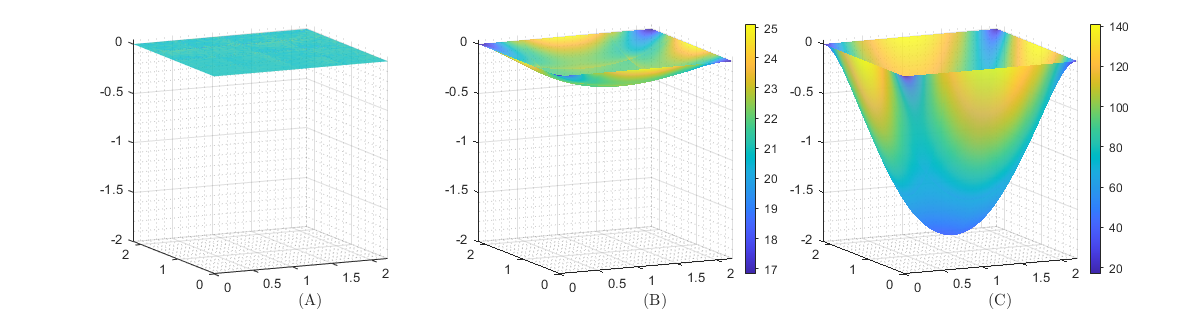
\includegraphics[scale = 0.6]{Images/mem_grav.png}
    \caption[Inflation of Square Sheet under Gravitational Loading]{Inflation of square sheet under gravitational loading: Configurations for $V = \{0, 0.6, 6\} V_{0}$. The colouring denotes the first invariant of stress.}
    \label{fig:mem_grav}
\end{figure}
\noindent Furthermore, the internal pressure is plotted against the enclosed volume in Figure \ref{fig:mem_pres} for various
 orders of approximating polynomials for the case of loading with volume constraint. The significant difference between
 the results of linear Lagrange elements as opposed to the higher-order elements is a result of the higher-order elements
 capturing the shape of the deformed structure more accurately. The relation of internal pressure and enclosed
 volume begins to converge to some solution for quadratic and quintic polynomials. 
\newpage
\begin{figure}[t]
    \centering
    \hspace*{-2cm}
    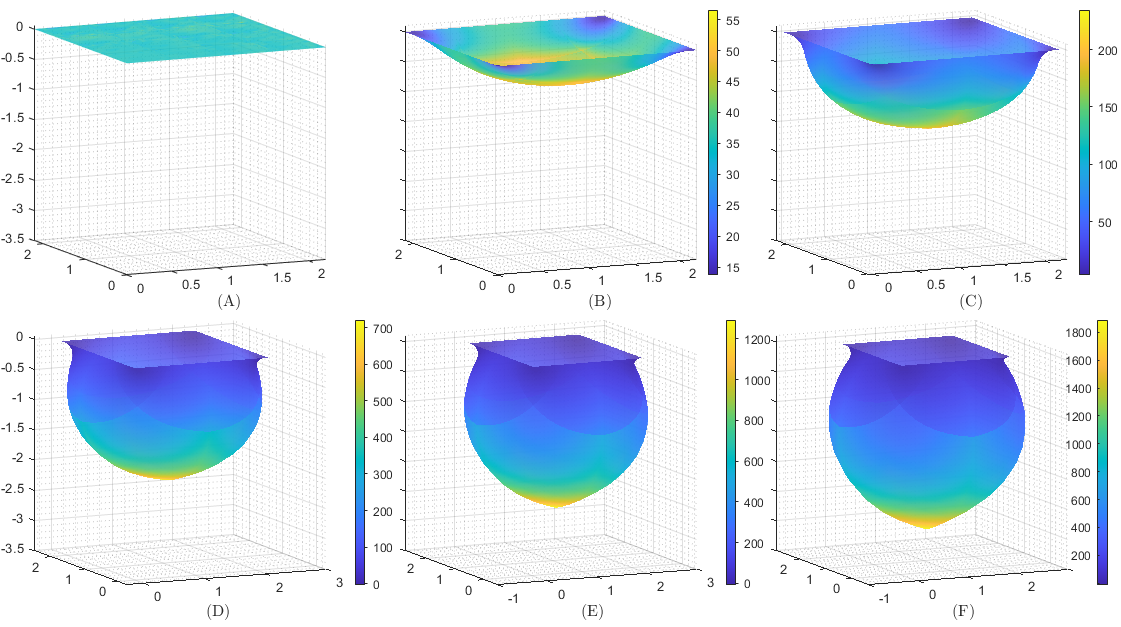
\includegraphics[scale = 0.65]{Images/mem_vol2.png}
    \caption[Inflation of Square Sheet with Volume Constraint]{Inflation of square sheet under loading with volume constraint: Configurations for $V = \{0, 2, 5, 10, 15, 20\} V_{0}$. The colouring denotes the first invariant of stress.}
    \label{fig:mem_vol}
\end{figure}
\begin{wrapfigure}{l}{0.5\textwidth}
    \centering
    \hspace*{-2cm}
    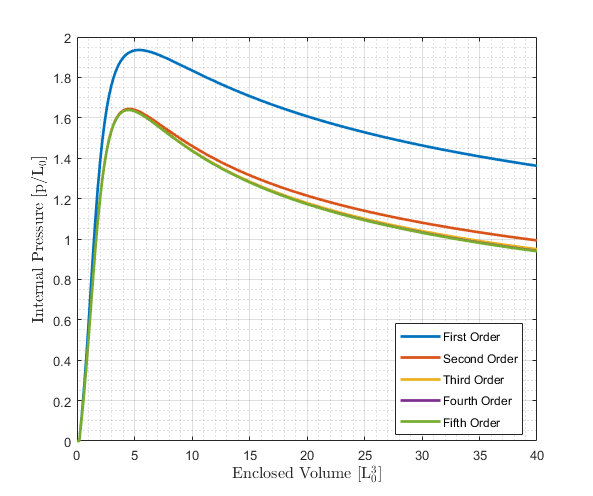
\includegraphics[scale = 0.60]{Images/mem_pres.png}
    \caption[Pressure-Volume Relation for Inflation of Square Sheet for Various Orders of Elements]{Internal pressure against volume for the inflation of square sheet}
    \label{fig:mem_pres}
\end{wrapfigure}
This is seen qualitatively in figure \ref{fig:mem_def} which shows the deformed sheet for a prescribed volume of $V=400V_0$ with 4x4 elements of various
 orders. With increasing order of the used approximation polynomial, the deformed configuration becomes smoother. For quadratic
 and cubic elements, the highest value of the first invariant of the stress tensor is found at a pronounced 'peak' at
 the bottom. Whereas in the quantic elements it disappears altogether, giving a smooth representation of the deformed structure.
 Based on this observation, one can state that the higher-order elements can represent the problem more accurately and closer
 to reality. Further improvements to the current framework can be achieved by using different
 approximation polynomials like isogeometric shape functions as can be seen in \cite{sauer2014}.
 \begin{figure}[h]
    \centering
    \begin{subfigure} [h] {0.48\textwidth}
        \hspace*{-3cm}
        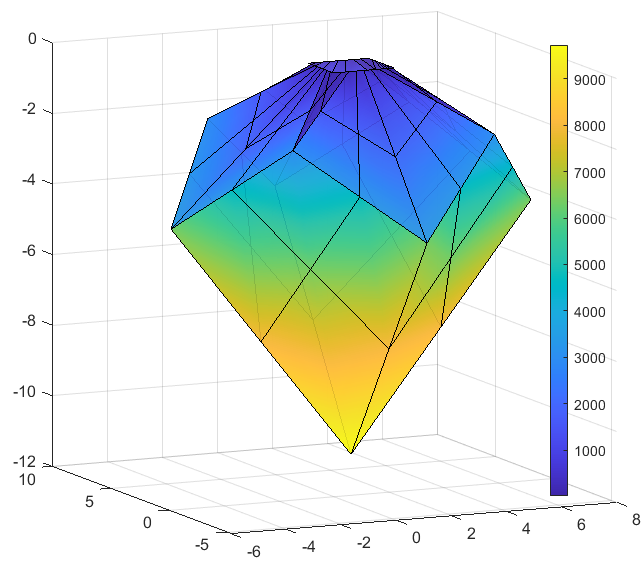
\includegraphics[scale = 0.55]{Images/mem_def1.png}
        \caption[]{4x4 linear elements}
        \label{fig:mem_def1}
    \end{subfigure}
    \hfill
    \begin{subfigure} [h] {0.48\textwidth}
        \hspace*{-.25cm}
        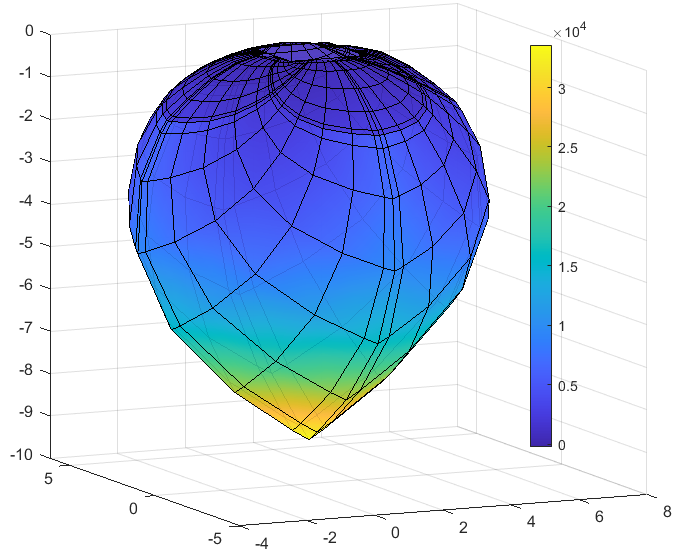
\includegraphics[scale = 0.55]{Images/mem_def2.png}
        \caption[]{4x4 quadratic elements}
        \label{fig:mem_def2}
    \end{subfigure}
    \\
    \begin{subfigure} [h] {0.48\textwidth}
        \hspace*{-3cm}
        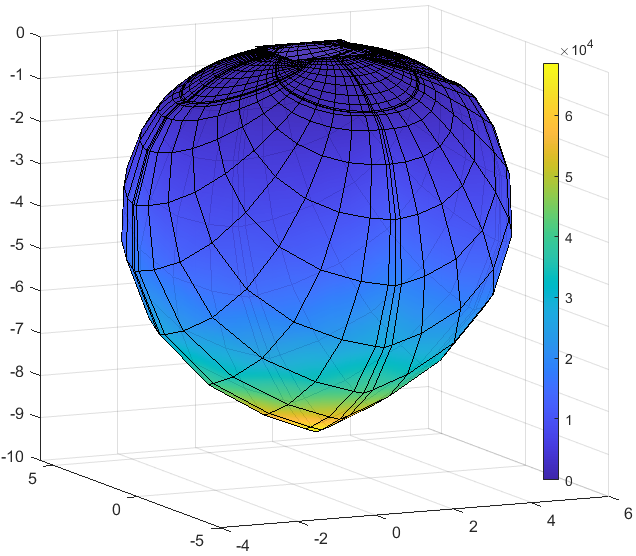
\includegraphics[scale = 0.55]{Images/mem_def3.png}
        \caption[]{4x4 cubic elements}
        \label{fig:mem_def3}
    \end{subfigure}
    \hfill
    \begin{subfigure} [h] {0.48\textwidth}
        \hspace*{-.25cm}
        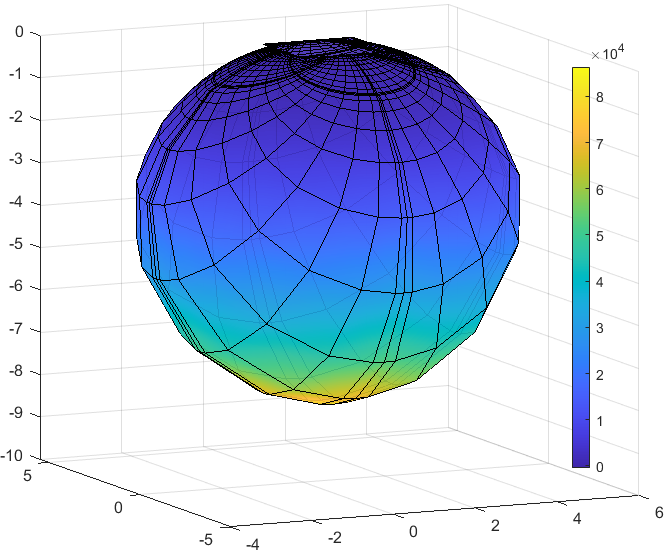
\includegraphics[scale = 0.55]{Images/mem_def5.png}
        \caption[]{4x4 quintic elements}
        \label{fig:mem_def5}
    \end{subfigure}
    \caption[Large Deformation of Square Sheet using Various Orders of Elemets]{Inflated square sheet: $V = 400 V_{0}$}
    \label{fig:mem_def}
\end{figure}


 \afterpage{\blankpage}
\chapter{Conclusion}
\label{Chapter5}

A general nonlinear framework for the solution of rotation-free solid membranes is presented. The theory in Section \ref{Chapter2} details
 the solution of general elliptic partial differential equations using the Finite Element Method. The function spaces of the test
 and trial functions are introduced for the well-posedness of the weak formulation necessary for a meaningful solution of the
 boundary value problem. Dirichlet, Neumann, and mixed boundary conditions are considered and the isoparametric parametric concept
 along with numerical quadrature is used to simplify the implementation of the solution on MATLAB. Section \ref{Chapter3} develops a
 nonlinear framework for the solution of problems involving large deformations of beams in a Euclidean basis. Discretisation of
 general kinematical quantities, balance laws, and constitution is introduced. The resulting nonlinear system of equations is solved using the Newton-Raphson method. 
 This framework is validated using simple numerical examples while comprehensively covering the load and displacement driven boundary conditions. 
 After a thorough development of the foundation, Section \ref{Chapter4} extends the previous chapters to develop the framework for curved structures.
 Based on the differential geometry of curved surfaces, the resulting framework is general, accounts for large deformations, and general material laws.
 The use of curvilinear coordinates further eases computation as the resulting formulation only uses three degrees of freedom, avoids the use
 of a local cartesian coordinate system, the transformation of derivatives, and allows the splitting of the strong and weak forms
 into the in-plane and out-of-plane parts allowing an easy extension of the framework to liquid membranes. The solution of the final nonlinear system
 is conducted using the theory developed in the previous chapters with the volume constraints being included in the system using
 the Lagrange multiplier method. This framework is validated through the consideration of the inflation of a square sheet. It is expected
 that the MATLAB implementation of the formuation will be able to reproduce the results of \cite{sauer2014} in the future. 

% Appendix 
\appendix % Cue to tell LaTeX that the following "chapters" are Appendices

% Include the appendices of the thesis as separate files from the Appendices folder
% Uncomment the lines as you write the Appendices

% Appendix A

\chapter{Nonlinear Framework} % Main appendix title

\label{AppendixA} % For referencing this appendix elsewhere, use \ref{AppendixA}


\section{Material Model Expressed in \emph{\textbf{S}}}
    Given the Cauchy stress tensor \eqref{neo_hookean_definition} and the definition of the Second
     Piola-Kircchhof stress tensor,~\eqref{eq:19} can be written as,
    \begin{equation}
        \begin{split}
        {\boldsymbol{S}} &= {J \boldsymbol{F^{-1}}} \left[ \frac{\mu}{J} \left(\boldsymbol{b} - \boldsymbol{I}\right) + \frac{\Lambda}{J}\ln{J}\boldsymbol{I}\right] \boldsymbol{F^{-T}}\\
        &= {J}  {\left[ \frac{\mu}{J} \left(\boldsymbol{F^{-1}b} - \boldsymbol{F^{-1}}\right) + \frac{\Lambda}{J}\ln{J}\boldsymbol{F^{-1}}\right] \boldsymbol{F^{-T}}}\\
        &= {J} {\left[ \frac{\mu}{J} \left(\boldsymbol{F^{-1}}\left(\boldsymbol{FF^T}\right) - \boldsymbol{F^{-1}}\right) + \frac{\Lambda}{J}\ln{J}\boldsymbol{F^{-1}}\right]} \boldsymbol{F^{-T}}\\ 
        &= {J} {\left[ \frac{\mu}{J} \left(\boldsymbol{F^T} - \boldsymbol{F^{-1}} \right) \boldsymbol{F^{-T}} + \frac{\Lambda}{J} \ln{J}\boldsymbol{F^{-1}F^{-T}} \right]}\\ 
        &= \mu \left( {\boldsymbol{F^TF^{-T}}} - \left( {\boldsymbol{F^TF}} \right)^{-1} \right) + \Lambda{\ln{J}\left(\boldsymbol{F^TF}\right)^{-1}}
        \end{split}
    \end{equation}
    
    \begin{equation}\label{S_neohookean}
        \therefore {\boldsymbol{S} = \mu\left(\boldsymbol{I} - \boldsymbol{C^{-1}}\right) + \Lambda\ln{J}\boldsymbol{C^{-1}}}
    \end{equation}
    %-------------------------------------------------------------------------------------------
\section{Derivation of Compliance Matrix in Reference Configuration}
    As the formulation assumes the existence of a cartesian basis, the right Cauchy-Green tensor and its inverse can be written, 
    \begin{equation} \label{eq:def_C_comp}
        \begin{split}
        {\boldsymbol{C}} &= {C^i_{.j}\, \boldsymbol{e}_i \otimes \boldsymbol{e}^j}\\
        {\boldsymbol{C}}^{-1} &= {\left(C^{-1}\right)^i_{.j} \boldsymbol{e}_i \otimes \boldsymbol{e}^j}.
        \end{split}
    \end{equation}
Writing~\eqref{S_neohookean} in indicial form using \eqref{eq:def_C_comp} and using the definition~\eqref{compliance_definition}
    \begin{equation} \label{eq:ref_comp_1}
        \begin{split}
            {S^i_{.j}} &= \mu {\left[\delta ^i_{.i} - \left(C^{-1}\right)^i_{.j}\right] + \Lambda \ln{J} \left(C^{-1}\right)^i_{.j}}\\
        {\Rightarrow 2\frac{\partial S^i_{.j}}{\partial C^a_{.b}}} &= 2\mu {\left[0 - \frac{\partial \left(C^{-1}\right)^i_{.j}}{\partial C^a_{.b}} \right] + 2\Lambda\frac{\partial \left(\ln{J}\left(C^{-1}\right)^i_{.j}\right)}{\partial C^a_{.b}}}\\
            &= 2\mu {\left[0 - \frac{\partial \left(C^{-1}\right)^i_{.j}}{\partial C^a_{.b}} \right] + 2\Lambda \left(C^{-1}\right)^i_{.j} \boldsymbol{e}_i \otimes \boldsymbol{e}^j \otimes \frac{\partial \left(\ln{J}\right)}{\partial C^a_{.b}} + 2\Lambda\ln{J} \frac{\partial \left(C^{-1}\right)^i_{.j}}{\partial C^a_{.b}}}\\
            &= {2\left(-\mu + \Lambda\ln{J}\right) \frac{\partial \left(C^{-1}\right)^i_{.j}}{\partial C^a_{.b}} + 2\Lambda\left(C^{-1}\right)^i_{.j} \boldsymbol{e}_i \otimes \boldsymbol{e}^j \otimes \left[\frac{1}{J} \frac{\partial J}{\partial C^a_{.b}}\right]}\\
        \implies \mathbb{C}^{i.a.}_{.j.b} &= 2\left(-\mu + \Lambda\ln{{J}}\right)\left({C}^{-1}\right)^{i}_{.a} \left({C}^{-1}\right)^{b}_{.j} + \Lambda {\left(C^{-1}\right)^i_{.j} \left(C^{-1}\right)^a_{.b}}
        \end{split}
    \end{equation}
%-------------------------------------------------------------------------------
\section{Derivation of Compliance Matrix in Current Configuration}
Given the expression of the compliance matrix in reference configuration
\begin{equation}\label{eq:22}
    \mathbb{C} = 2\left(-\mu + \Lambda\ln{J}\right)\left(C^{-1}\right)^i_{.a} \left(C^{-1}\right)^b_{.j} \boldsymbol{e}_{i} \otimes \boldsymbol{e}^{a} \otimes \boldsymbol{e}_{b} \otimes \boldsymbol{e}^{j}
    + \Lambda \left(C^{-1}\right)^i_{.j} \left(C^{-1}\right)^a_{.b} \boldsymbol{e}_{i} \otimes \boldsymbol{e}^{j} \otimes \boldsymbol{e}_{a} \otimes \boldsymbol{e}^{b}.
\end{equation}
\normalsize and using the push-forward transformation to transform \eqref{eq:22} to the current configuration
\begin{equation}
    \begin{split}
    \mathbbmss{c} &= 2\left(-\mu + \Lambda\ln{J}\right)\left(C^{-1}\right)^i_{.a} \left(C^{-1}\right)^b_{.j} 
    \left(\boldsymbol{F\, e}_i \otimes \boldsymbol{e}^a \, \boldsymbol{F}^T\right) \otimes \left(\boldsymbol{F\,e}_b \otimes \boldsymbol{e}^j \,\boldsymbol{F^T}\right)\\
    &+ \Lambda \left(C^{-1}\right)^i_{.j} \left(C^{-1}\right)^a_{.b} \left(\boldsymbol{F\,e}_i \otimes \boldsymbol{e}^j \,\boldsymbol{F}^T\right) \otimes \left(\boldsymbol{F\,e}_a \otimes \boldsymbol{e}^b\, \boldsymbol{F}^T\right)\\
    &:= \mathbb{I} + \mathbb{II}
    \end{split}
\end{equation}
\normalsize Operating on $\mathbb{I}$
\begin{equation} \label{eq:I}
    \begin{split}
        \mathbb{I} &= 2\left(-\mu + \Lambda\ln{J}\right)\left(C^{-1}\right)^i_{.a} \left(C^{-1}\right)^b_{.j} \\
        &\quad \left[F^p_{.q} \, \boldsymbol{e}_p \,(\boldsymbol{e}^q \cdot \boldsymbol{e}_i)\right] \otimes \left[(\boldsymbol{e}^a \cdot \boldsymbol{e}_r)\, \boldsymbol{e}^s \left(F^T\right)^r_{.s}\right] \left[F^t_{.u} \,\boldsymbol{e}_t \,(\boldsymbol{e}^u \cdot \boldsymbol{e}_b)\right] \otimes \left[(\boldsymbol{e}^j \cdot \boldsymbol{e}_v) \,\boldsymbol{e}^w \left(F^T\right)^v_{.w} \right]\\
        &= 2\left(-\mu + \Lambda\ln{J}\right) \left(F^{-1}F^{-T}\right)^i_{.a} \left(F^{-1}F^{-T}\right)^b_{.j} \left[F^p_{.q} \: \delta^q_{.i} \: \delta^a_{.r} \: (F^T)^r_{.s} \: F^t_{.u} \: \delta^u_{.b} \: \delta^j_{.v} \: (F^T)^v_{.w} \right] \boldsymbol{e}_p \otimes \boldsymbol{e}^s \otimes \boldsymbol{e}_t \otimes \boldsymbol{e}^w\\
        \mathbb{I}^{p\,.\,s\,.}_{\,.\,w\,.\,t} & = 2\left(-\mu + \Lambda\ln{J}\right) \left(F^{-1}\right)^i_{.c} \left(F^{-T}\right)^c_{.a} \left(F^{-1}\right)^b_{.d} \left(F^{-T}\right)^d_{.j} \left[F^p_{.i} \: \delta^a_{.r} \: (F^T)^r_{.s} \: F^t_{.b} \: \delta^j_{.v} \: (F^T)^v_{.w}\right]\\
        & = 2\left(-\mu + \Lambda\ln{J}\right)\left[ F^p_{.i} \: (F^{-1})^i_{.c} \: F^t_{.b} \: (F^{-1})^b_{.d}\right] \left[(F^{-T})^c_{.a} \: \delta^a_{.r} \: (F^T)^r_{.s}\right] \left[(F^{-T})^d_{.j} \:  \delta^j_{.v} \: (F^T)^v_{.w}\right]\\
        & =  2\left(-\mu + \Lambda\ln{J}\right) \delta^p_{.c} \: \delta^t_{.d} \: (F^{-T})^c_{.r} \: (F^T)^r_{.s} \: (F^{-T})^d_{.v} \: (F^T)^v_{.w} \\
        &= 2\left(-\mu + \Lambda\ln{J}\right) \delta^p_{.c} \; \delta^t_{.d} \; \delta^c_{.s} \; \delta^d_{.w}\\
    \implies \mathbb{I} &= 2\left(-\mu + \Lambda\ln{J}\right) \delta^p_{.s} \; \delta^t_{.w} \; \boldsymbol{e}_p \otimes \boldsymbol{e}^s \otimes \boldsymbol{e}_t \otimes \boldsymbol{e}^w
    \end{split}
\end{equation}
Similarly for $\mathbb{II}$
\begin{equation} \label{eq:II}
    \begin{split}
        \mathbb{II} &= \frac{\Lambda}{2}\left(C^{-1}\right)^i_{.j} \left(C^{-1}\right)^a_{.b} \left[F^p_{.q}\, \boldsymbol{e}_p \,(\boldsymbol{e}^q \cdot \boldsymbol{e}_i)\right] \otimes \left[(\boldsymbol{e}^j \cdot \boldsymbol{e}_v) \,\boldsymbol{e}^w \left(F^T\right)^v_{.w}\right] \\
        &\quad \otimes\left[F^r_{.s}\, \boldsymbol{e}_r \,(\boldsymbol{e}^s \cdot \boldsymbol{e}_a)\right] \otimes \left[(\boldsymbol{e}^b \cdot \boldsymbol{e}_t)\, \boldsymbol{e}^u \left(F^T\right)^t_{.u} \right]\\
    &= \frac{\Lambda}{2} \left(C^{-1}\right)^i_{.j} \left(C^{-1}\right)^a_{.b} \left[F^p_{.q} \,\delta^q_{.i} \,\delta^j_{.v} \,(F^T)^v_{.w} \,F^r_{.s} \,\delta^s_{.a} \,\delta^b_{.t}\, (F^T)^t_{.u} \right] \boldsymbol{e}_p \otimes \boldsymbol{e}^w \otimes \boldsymbol{e}_r \otimes \boldsymbol{e}^u\\
    \mathbb{II}^{p\,.\,r\,.}_{\,.\,w\,.\,u} &= \frac{\Lambda}{2} \left(F^{-1}F^{-T}\right)^i_{.j} \left(F^{-1}F^{-T}\right)^a_{.b} \left[F^p_{.i} \,\delta^j_{.v}\, (F^T)^v_{.w} \,F^r_{.a} \,\delta^b_{.t} \,(F^T)^t_{.u} \right]\\
    &= \frac{\Lambda}{2} \left(F^{-1}\right)^i_{.c} \left(F^{-T}\right)^c_{.j} \left(F^{-1}\right)^a_{.d} \left(F^{-T}\right)^d_{.b} \left[F^p_{.i}\, \delta^j_{.v}\, (F^T)^v_{.w} \,F^r_{.a} \,\delta^b_{.t} \,(F^T)^t_{.u} \right]\\
    &= \frac{\Lambda}{2}(F^p_{.i} \, (F^{-1})^i_{.c})\,(F^r_{.a}\,(F^{-1})^a_{.d})\left[\left(F^{-T}\right)^c_{.j} \,\delta^j_{.v} \,(F^T)^v_{.w}\right] \left[\left(F^{-T}\right)^d_{.b} \,\delta^b_{.t} \,(F^T)^t_{.u}\right]\\
    &= \frac{\Lambda}{2} \delta^p_{.c} \: \delta^r_{.d} \: \left[(F^{-T})^c_{.v}\, (F^T)^v_{.w}\right] \left[(F^{-T})^d_{.t}\, (F^T)^t_{.u}\right]\\
    &= \frac{\Lambda}{2} \delta^p_{.c} \; \delta^r_{.d} \; \delta^c_{.w}\;  \delta^d_{.u} \; \boldsymbol{e}_p \otimes \boldsymbol{e}^w \otimes \boldsymbol{e}_r \otimes \boldsymbol{e}^u\\
    &= \frac{\Lambda}{2} \underbrace{\delta^p_{.w} \; \delta^r_{.u} \; \boldsymbol{e}_p \otimes \boldsymbol{e}^w \otimes \boldsymbol{e}_r \otimes \boldsymbol{e}^u}_{r \rightarrow s, u \rightarrow t}\\
\implies \mathbb{II} &= \frac{\Lambda}{2} \; \delta^p_{.w} \; \delta^s_{.t} \; \boldsymbol{e}_p \otimes \boldsymbol{e}^w \otimes \boldsymbol{e}_s \otimes \boldsymbol{e}^t
\end{split}
\end{equation}
\normalsize Using \eqref{eq:I} and \eqref{eq:II}, the compliance matrix in the current configuration in indicial form is
\begin{equation}
    \mathbbmss{c}^{p\,.\,s\,.}_{\,.\,w\,.\,t} = 2\left(-\mu + \Lambda\ln{J}\right) \delta^p_{.s} \;\delta^t_{.w} + \frac{\Lambda}{2} \delta^p_{.w} \; \delta^s_{.t}.
\end{equation}

\include{Appendix/AppendixB}
% Bibliography
\include{Bibliography/Bibliography}


\end{document}  
